\chapter{Разработка программно-аппаратного комплекса для генерации персонажа D\&D и тестирование работоспособности прототипа устройства}

\section{Разработка программного обеспечения для генерации персонажа D\&D}

Программа, которая будет являться прошивкой микроконтроллера должна выполнять все требования к генератору, описанные в предыдущей главе к которым относятся следующие:

\begin{enumerate}
    \item Выбор расы персонажа.
    \item Выбор класса персонажа.
    \item Генерация значений 5 базовых характеристик:
    \begin{enumerate}
        \item Сила (Strong --- сокращенно <<Str>>).
        \item Телосложение (Constitution --- сокращенно <<Con>>).
        \item Ловкость (Dexterity --- сокращенно <<Dex>>).
        \item Интеллект (Intelligence --- сокращенно <<Int>>).
        \item Мудрость (Wisdom --- сокращенно <<Wis>>).
        \item Харизма (Charisma --- сокращенно <<Cha>>).
    \end{enumerate}
    \item Расчет значений для ряда побочных характеристик: класс защиты и хит-поинтов персонажа (на основе базовых характеристик).
    \item Выбор снаряжения на основе ранее выбранных игроком характеристик.
\end{enumerate}

Поскольку для вывода информации служит LCD-дисплей, то в генераторе также должно быть реализовано понятное текстовое меню для вывода информации о персонаже. 

Структура меню генератора персонажа следующая:

\begin{enumerate}
    \item Приветственный экран.
    \item Меню выбора расы персонажа.
    \item Меню выбора класса персонажа.
    \item Экран с выводом выбранных расы и класса, а также со значениями рассчитанных характеристик.
\end{enumerate}

Переключение между пунктами меню осуществляется с помощью кнопок, нажатие которых обрабатывается.

Для реализации данного набора возможностей решение было разбито на функции, каждая из которых отвечает за выбор параметров персонажа или за генерацию значений его характеристик.

\subsection*{Функция mainText}

Эта функция представляет собой реализацию приветственного окна, в котором сообщается о назначении программы (<<Character generator D\&D>>) и указывается, что для продолжения работы нужно нажать соответствующую кнопку (<<SELECT>>).

Помимо этого, после нажатия кнопки внутри функции генерируются псевдослучайные числа, которые имитируют броски игральной кости. Генерируется четыре псевдослучайных числа и находится сумма этих чисел, исключая меньшее. Такие манипуляции производятся шесть раз (по количеству характеристик персонажа). Блок-схема подпрограммы mainText изображена на рис.~\ref{fig:main1},~\ref{fig:main2}.

\begin{figure}[H]
    \centering
    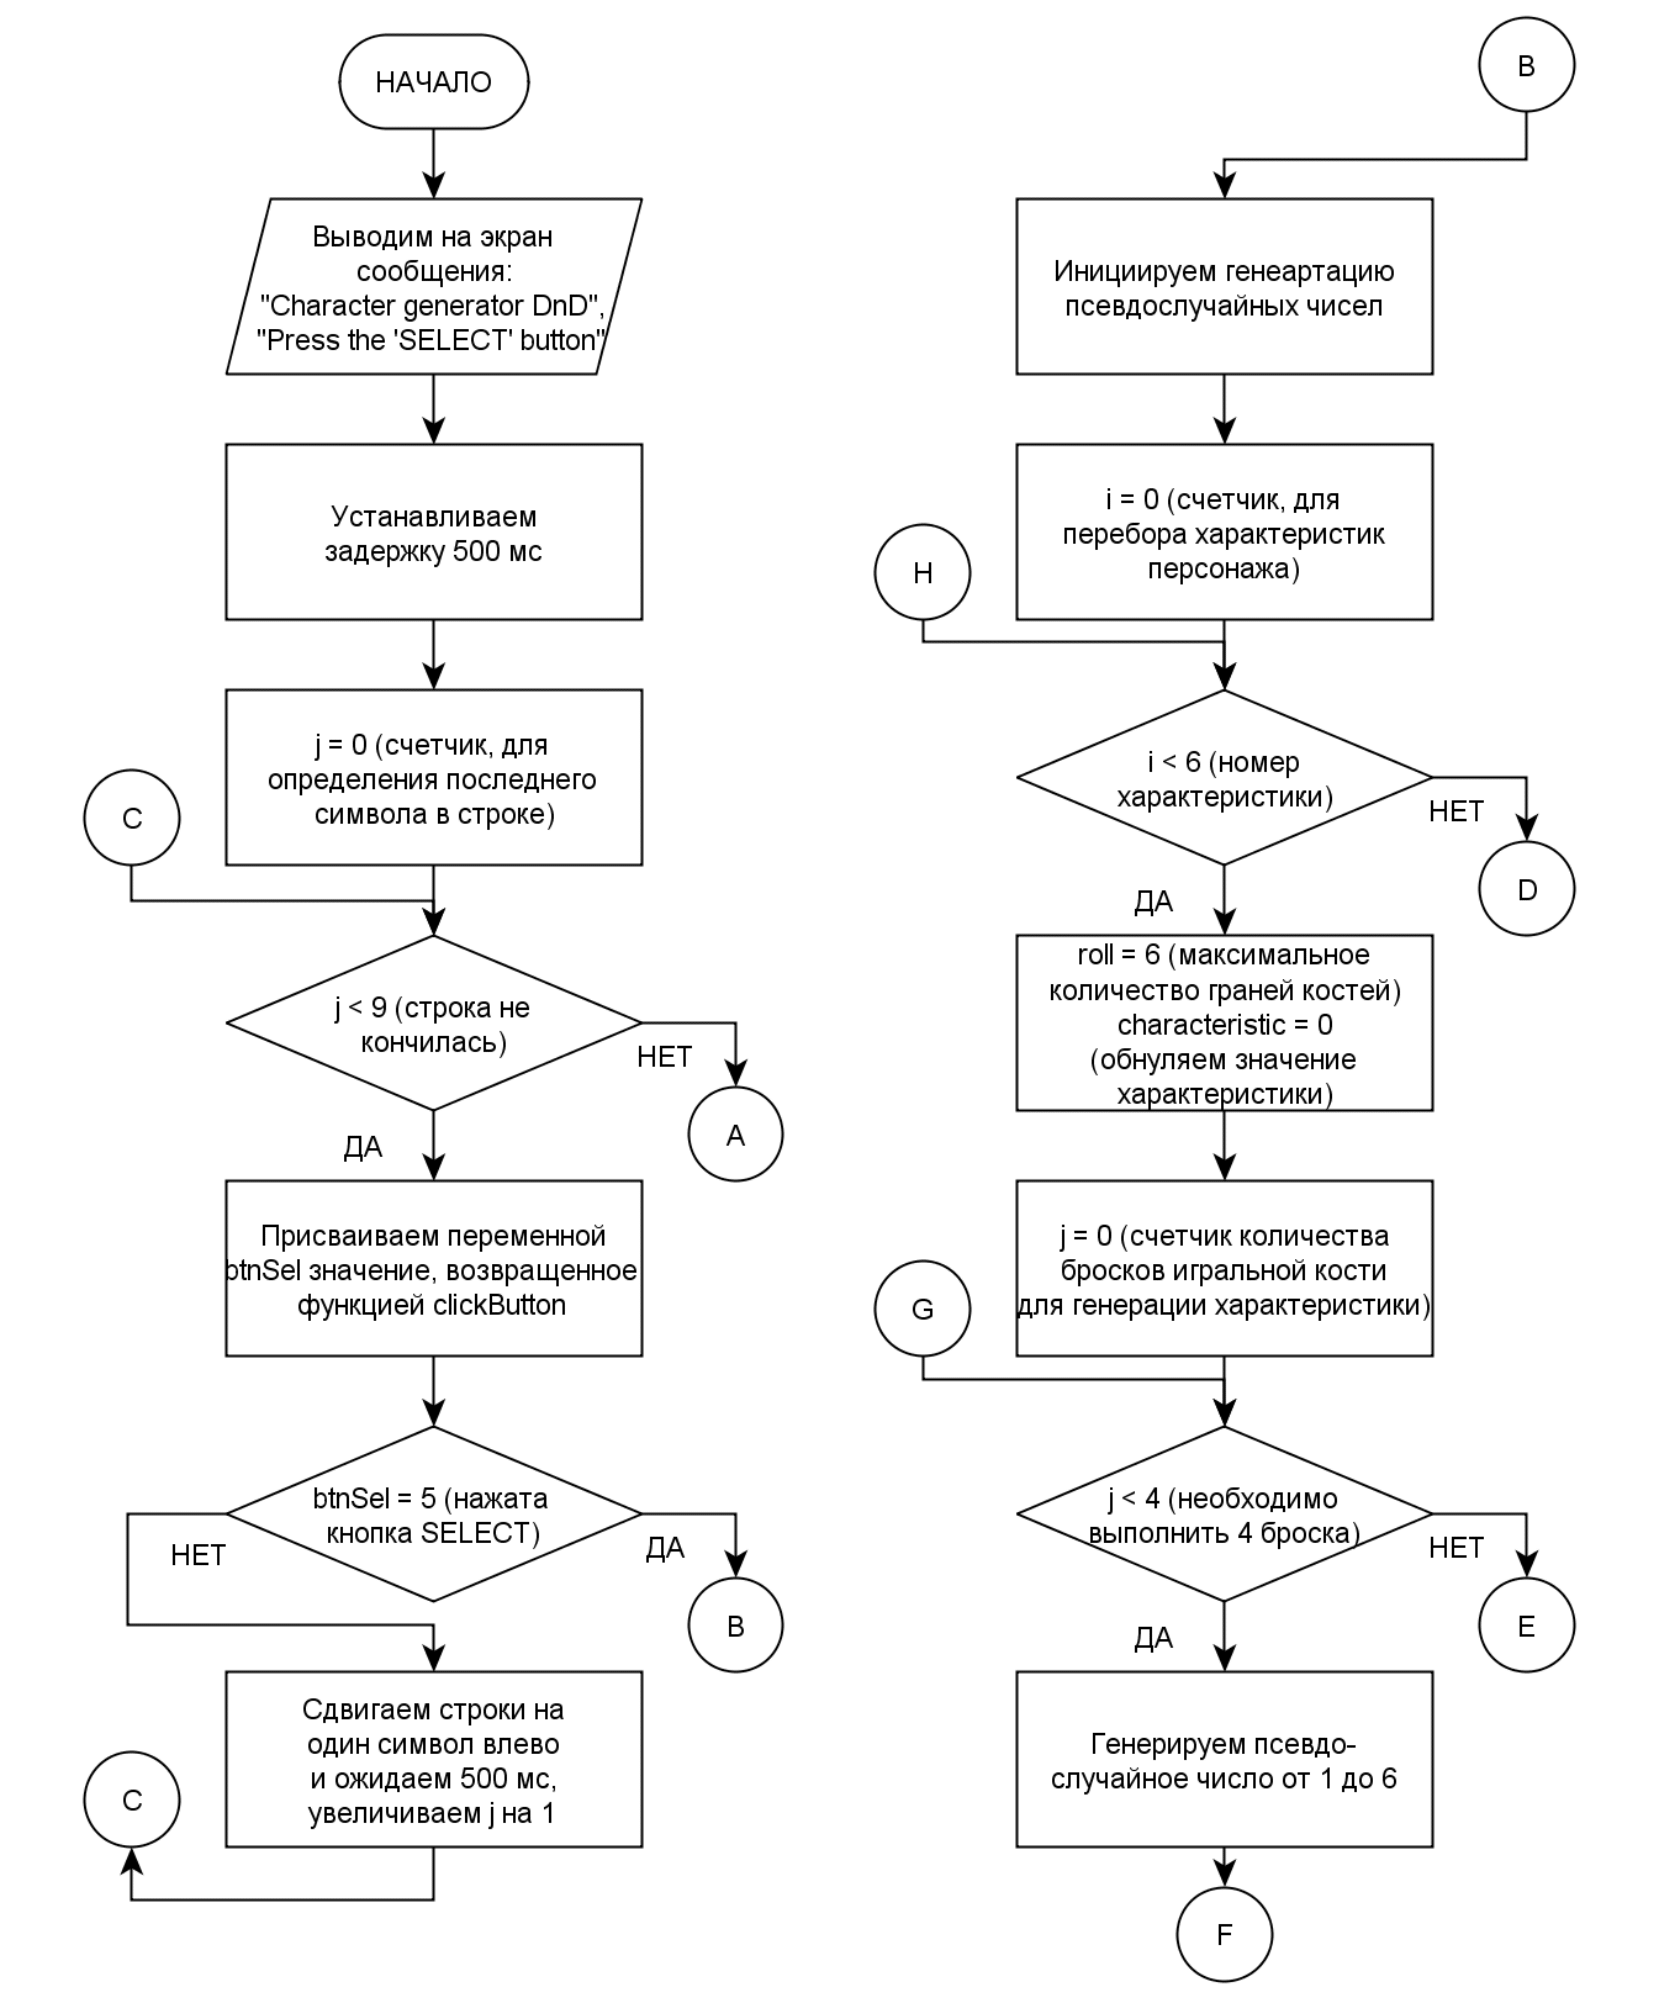
\includegraphics[scale=0.75]{mainText1.png}
    \caption{Блок-схема функции mainText.}
    \label{fig:main1}
\end{figure}

\begin{figure}[H]
    \centering
    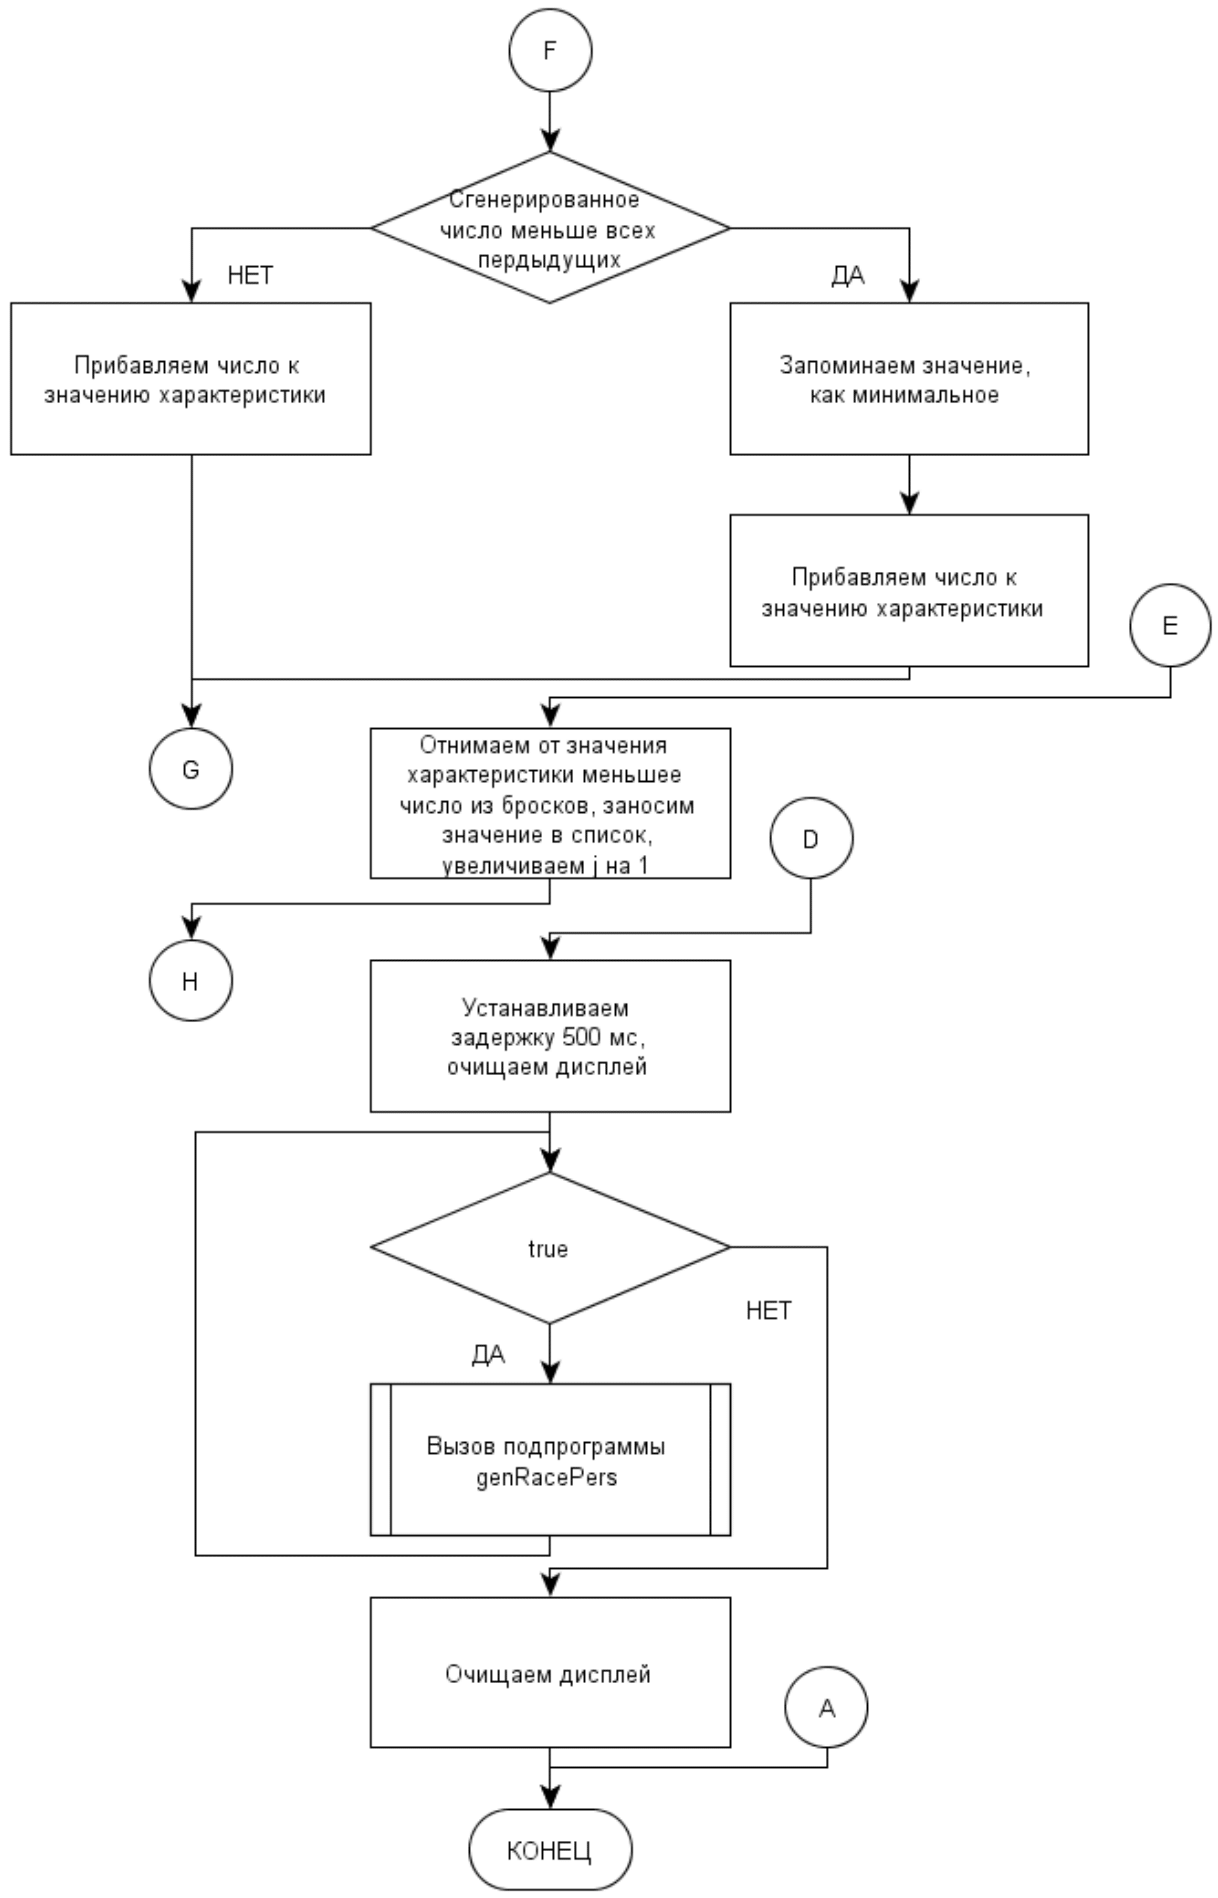
\includegraphics[scale=1]{mainText2.png}
    \caption{Блок-схема функции mainText.}
    \label{fig:main2}
\end{figure}

\subsection*{Функция genRacePers}

В этой функции реализована часть генератора, которая отвечает за выбор пользователем расы персонажа. На экран выводятся двенадцать вариантов рас, среди которых пользователь может переключаться нажатием на кнопки: <<ВВЕРХ>> (<<UP>>), <<ВНИЗ>> (<<DOWN>>), <<ВПРАВО>> (<<RIGHT>>), <<ВЛЕВО>> (<<LEFT>>); чтобы подтвердить свой выбор требуется нажать кнопку <<ВЫБРАТЬ>> (<<SELECT>>). Блок-схема подпрограммы genRacePers (см. рис.~\ref{fig:race1},~\ref{fig:race2}).

\begin{figure}[H]
    \centering
    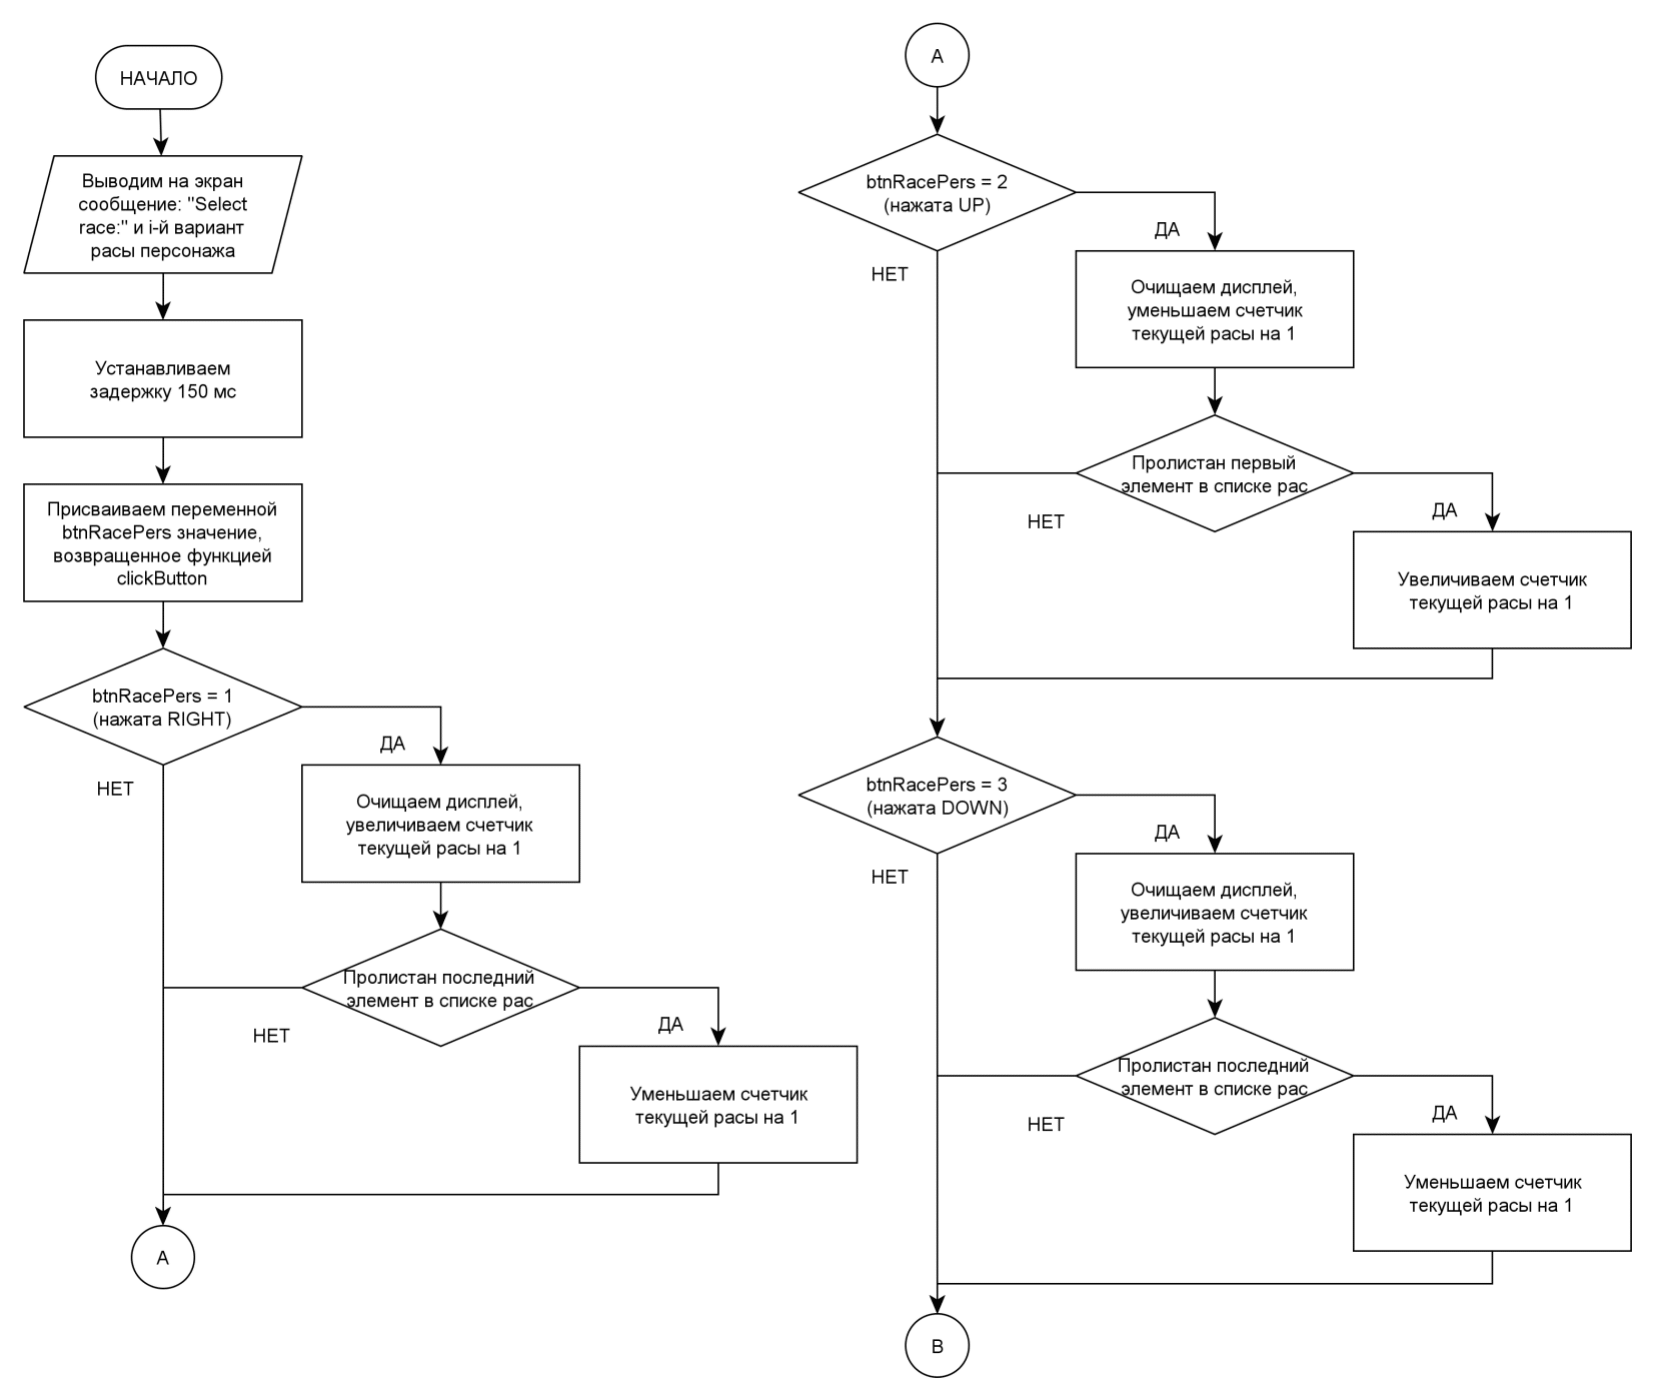
\includegraphics[scale=0.75]{genRacePers1.png}
    \caption{Блок-схема функции genRacePers.}
    \label{fig:race1}
\end{figure}

\begin{figure}[H]
    \centering
    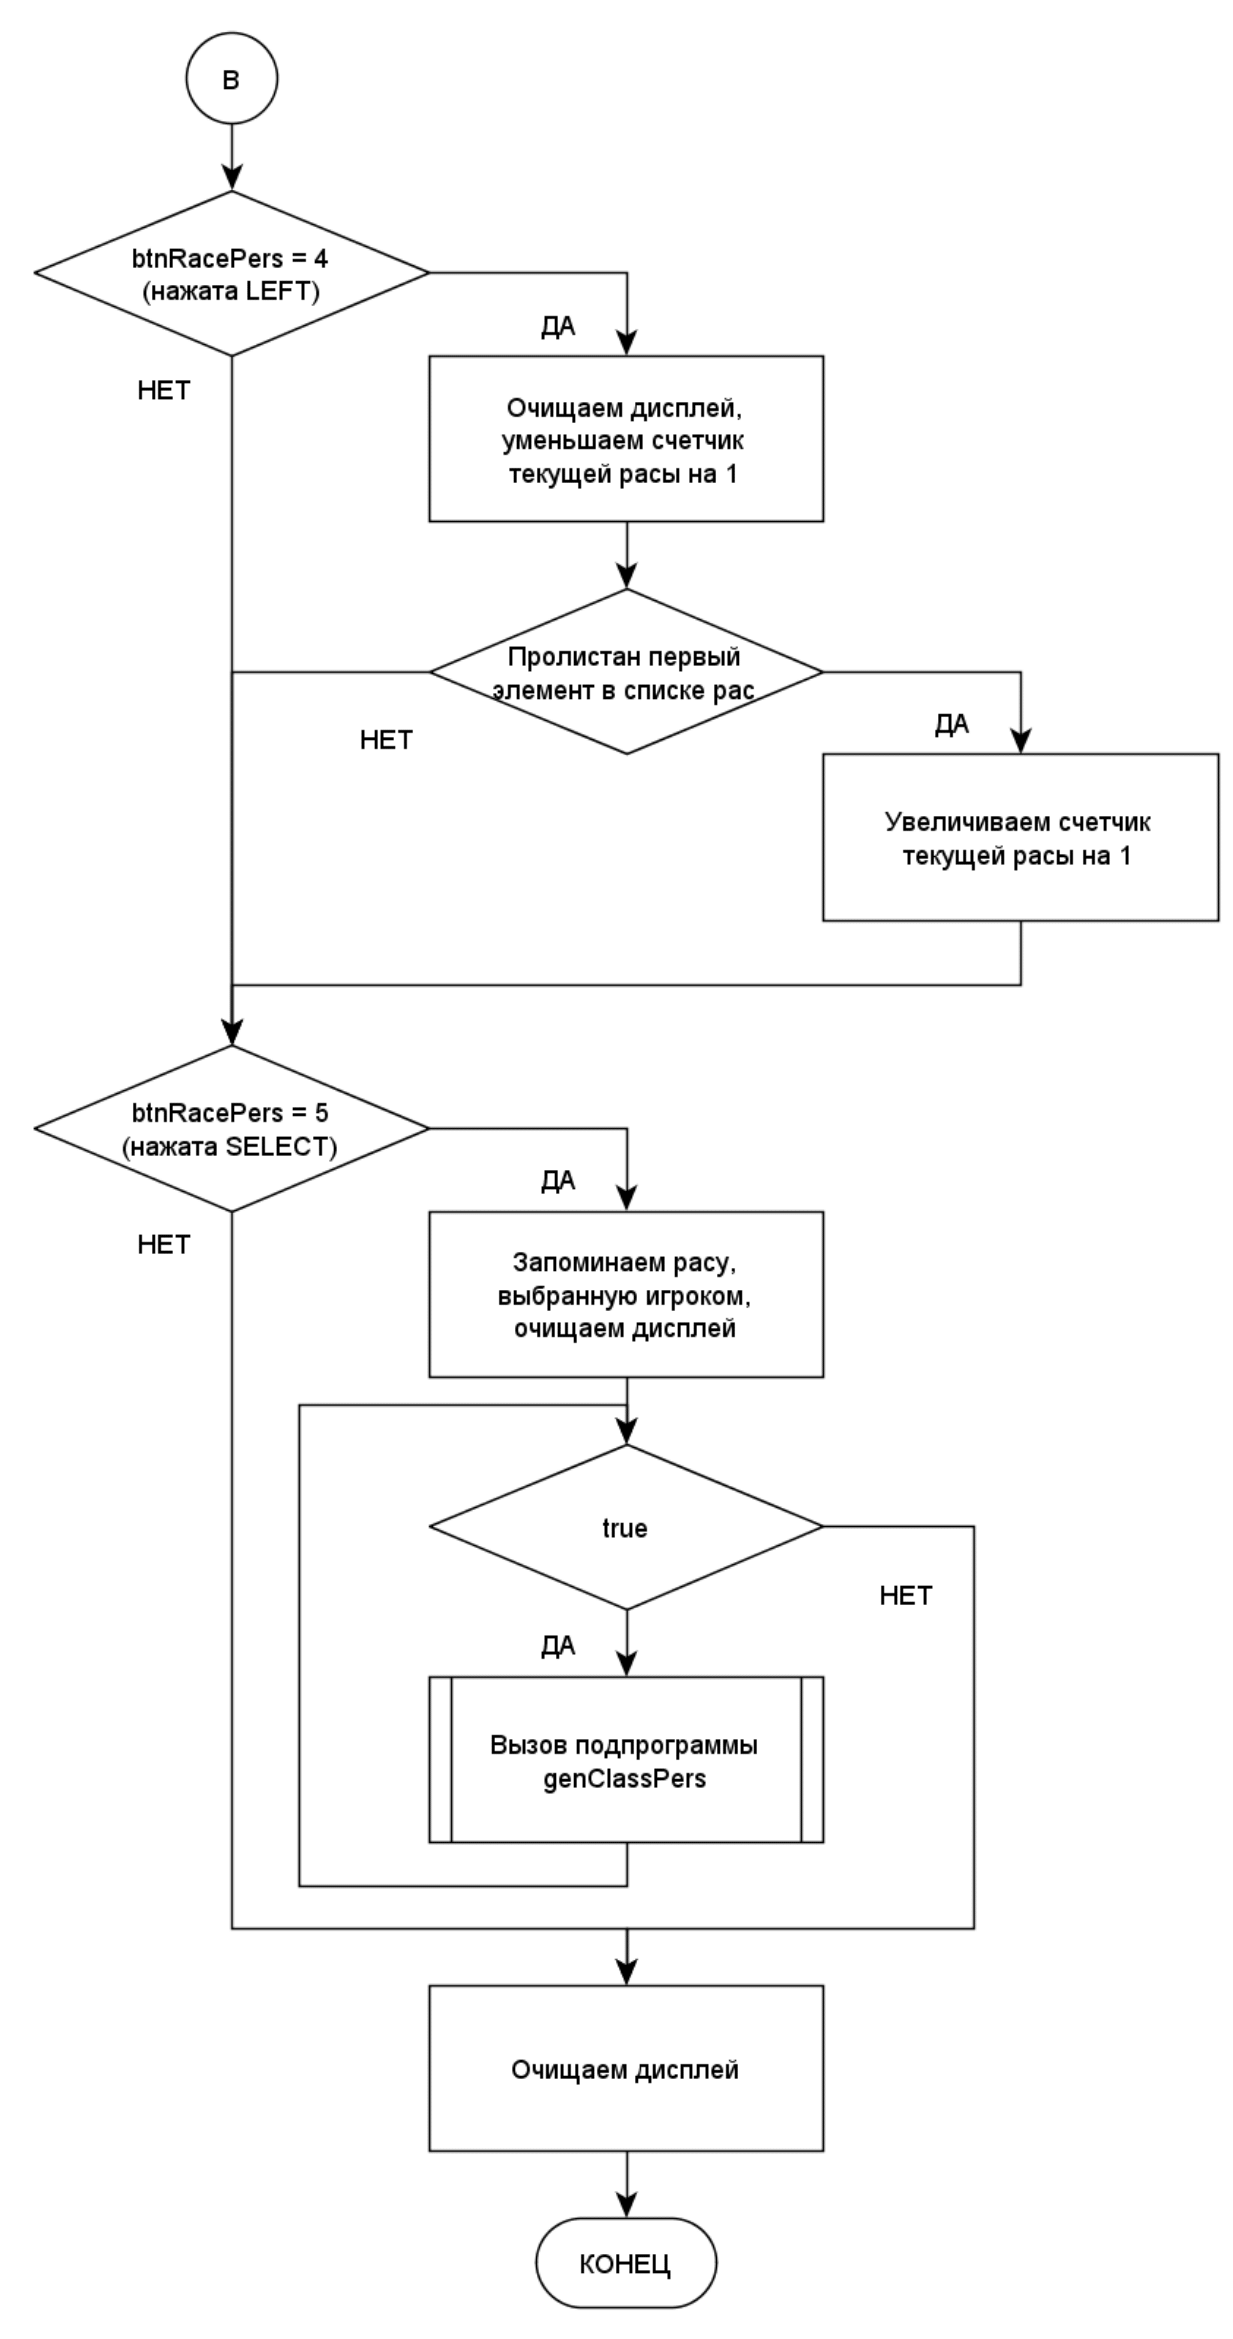
\includegraphics[scale=0.8]{genRacePers2.png}
    \caption{Блок-схема функции genRacePers.}
    \label{fig:race2}
\end{figure}

\subsection*{Функция genClassPers}

В этой функции реализована возможность выбора класса персонажа. На экран последовательно выводятся тринадцать предусмотренных классов, между которыми также можно переключаться с помощью кнопок, для подтверждения выбора предусмотрена кнопка <<ВЫБРАТЬ>> (<<SELECT>>). Блок-схема подпрограммы genClassPers изображена на рис.~\ref{fig:class1},~\ref{fig:class2}.

\begin{figure}[H]
    \centering
    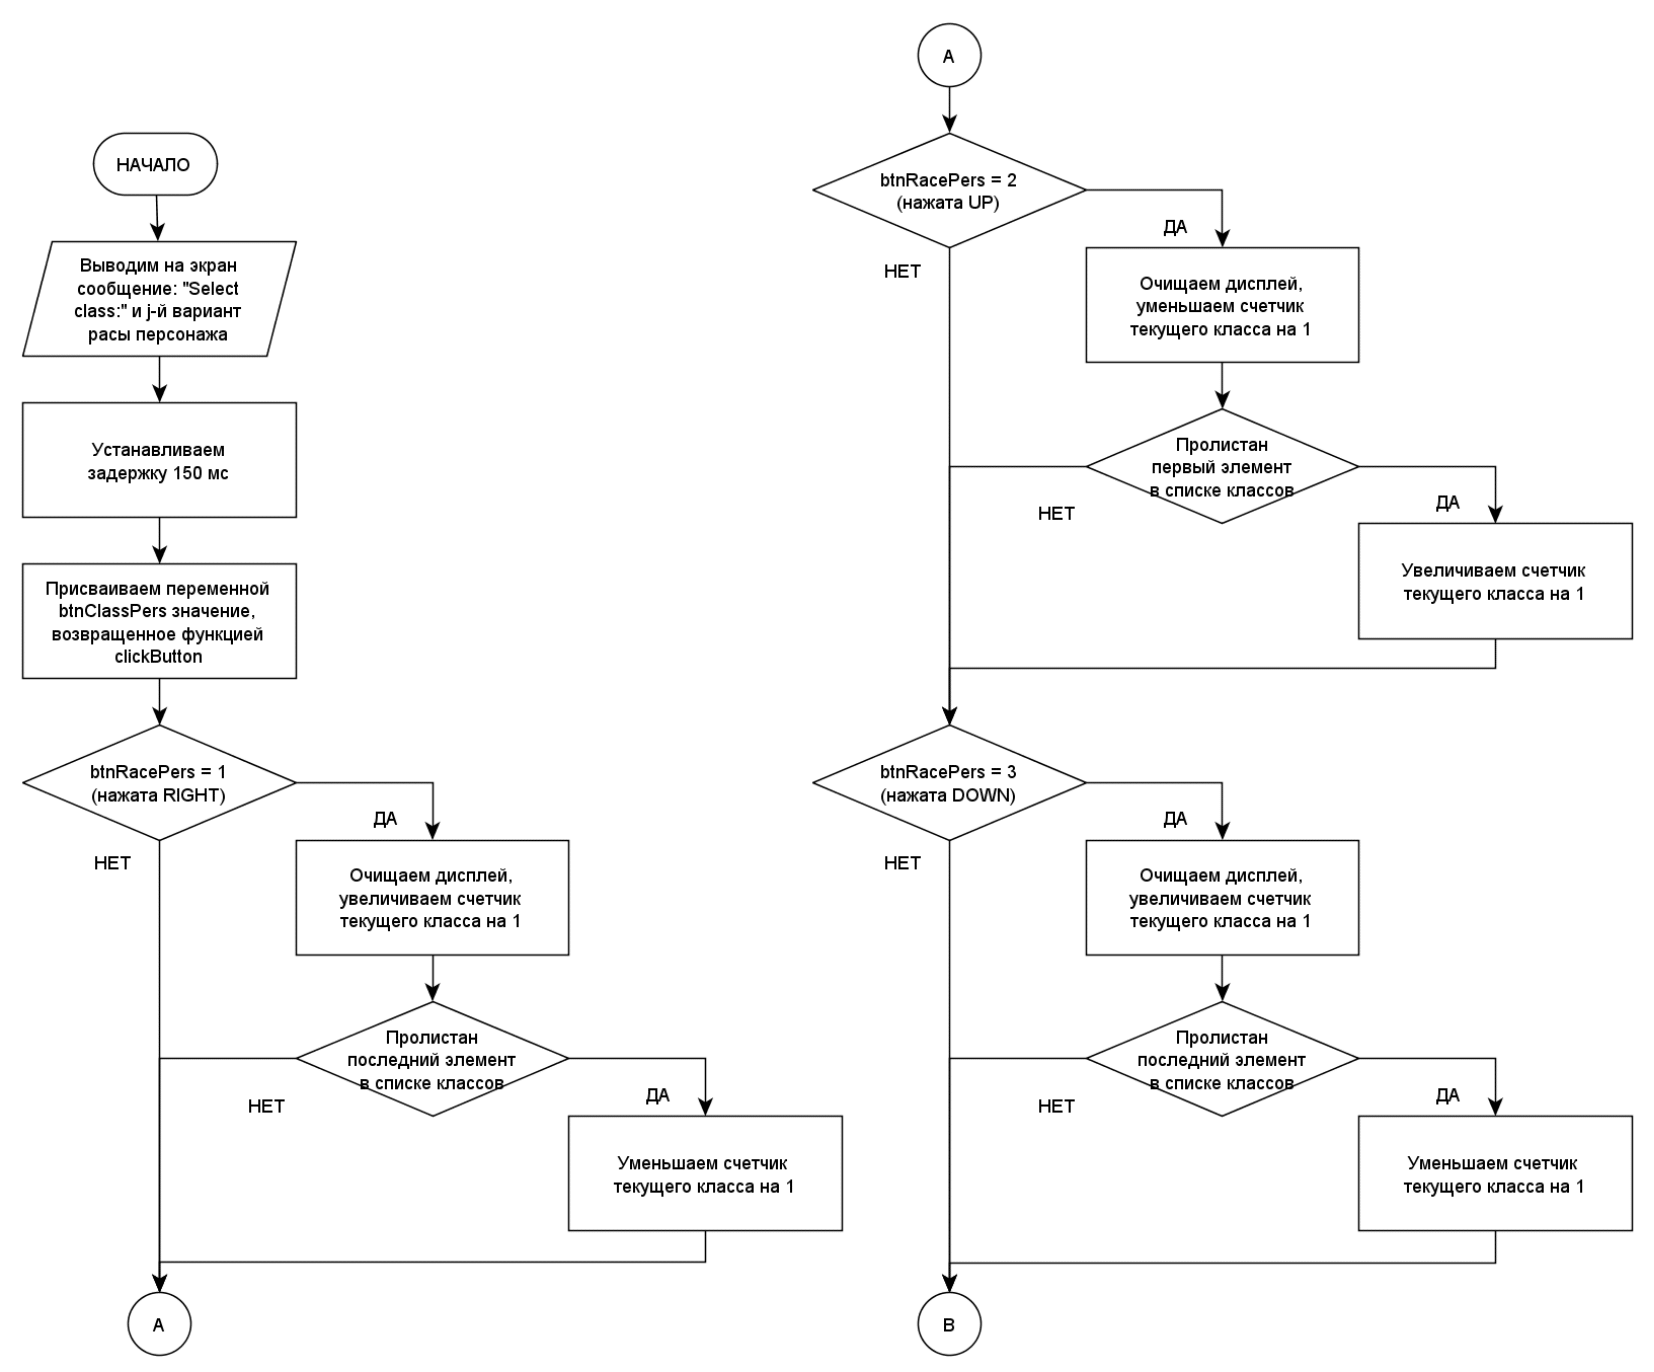
\includegraphics[scale=0.75]{genClassPers1.png}
    \caption{Блок-схема функции genClassPers.}
    \label{fig:class1}
\end{figure}

\begin{figure}[H]
    \centering
    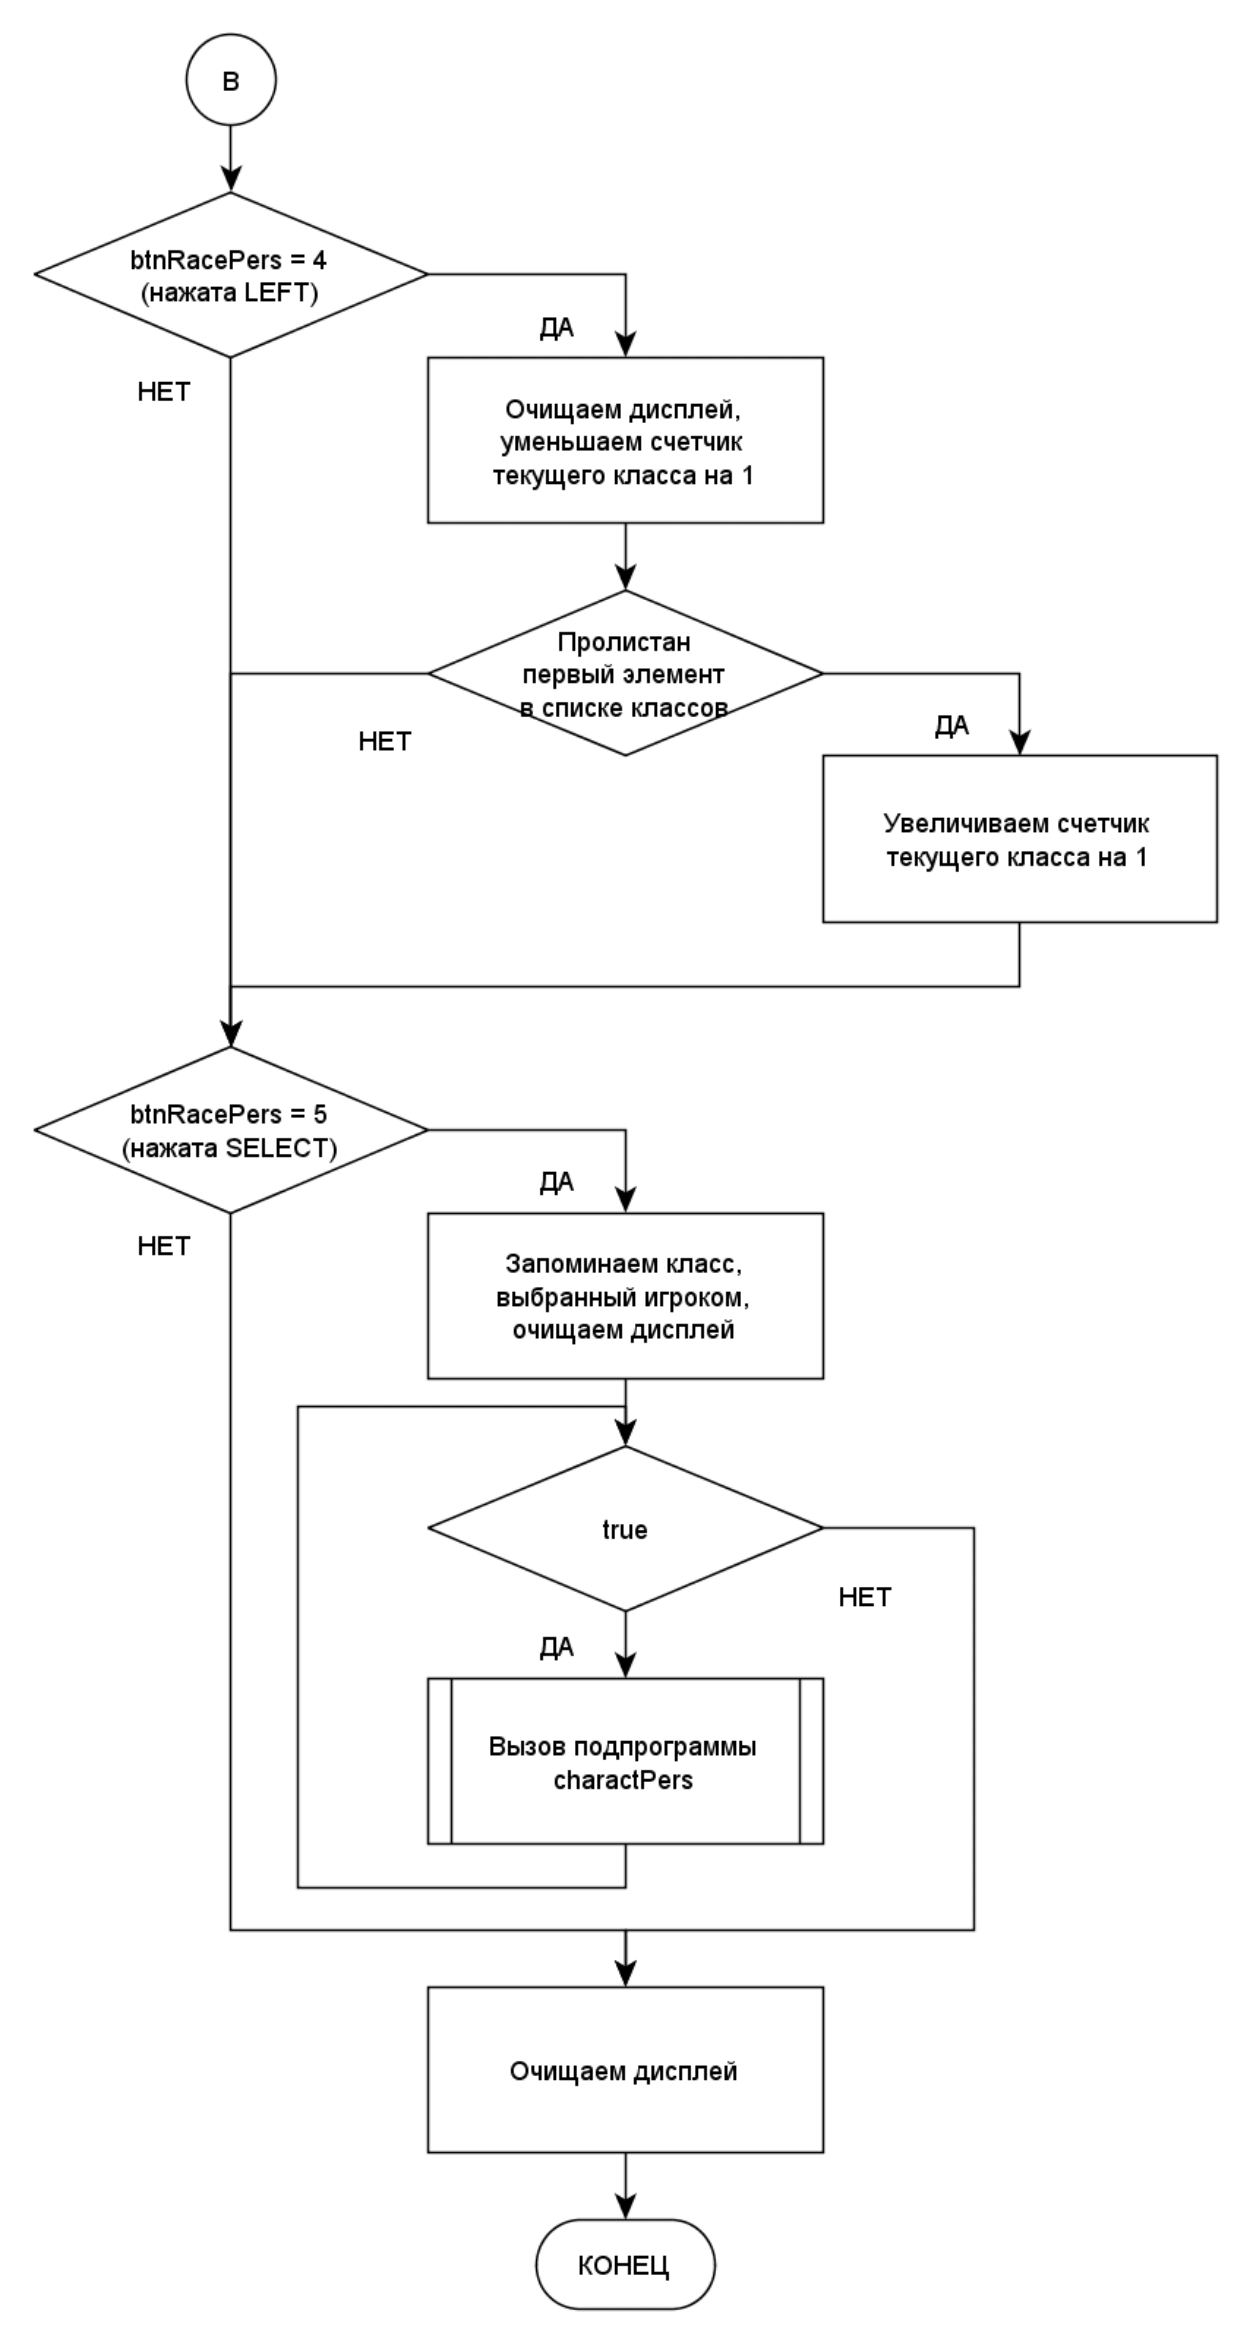
\includegraphics[scale=0.8]{genClassPers2.png}
    \caption{Блок-схема функции genClassPers.}
    \label{fig:class2}
\end{figure}

\subsection*{Функция charactPers}

С помощью данной функции на экран выводятся значения характеристик, сгенерированные в функции mainText, а также на их основе высчитываются количество хит-поинтов и класс защиты для выбранных расы и класса, которые также выводятся на экран. Навигация здесь, также как и в предыдущих функциях осуществляется с помощью кнопок. Блок-схема подпрограммы charactPers изображена на рис.~\ref{fig:char1},~\ref{fig:char2}.

\begin{figure}[H]
    \centering
    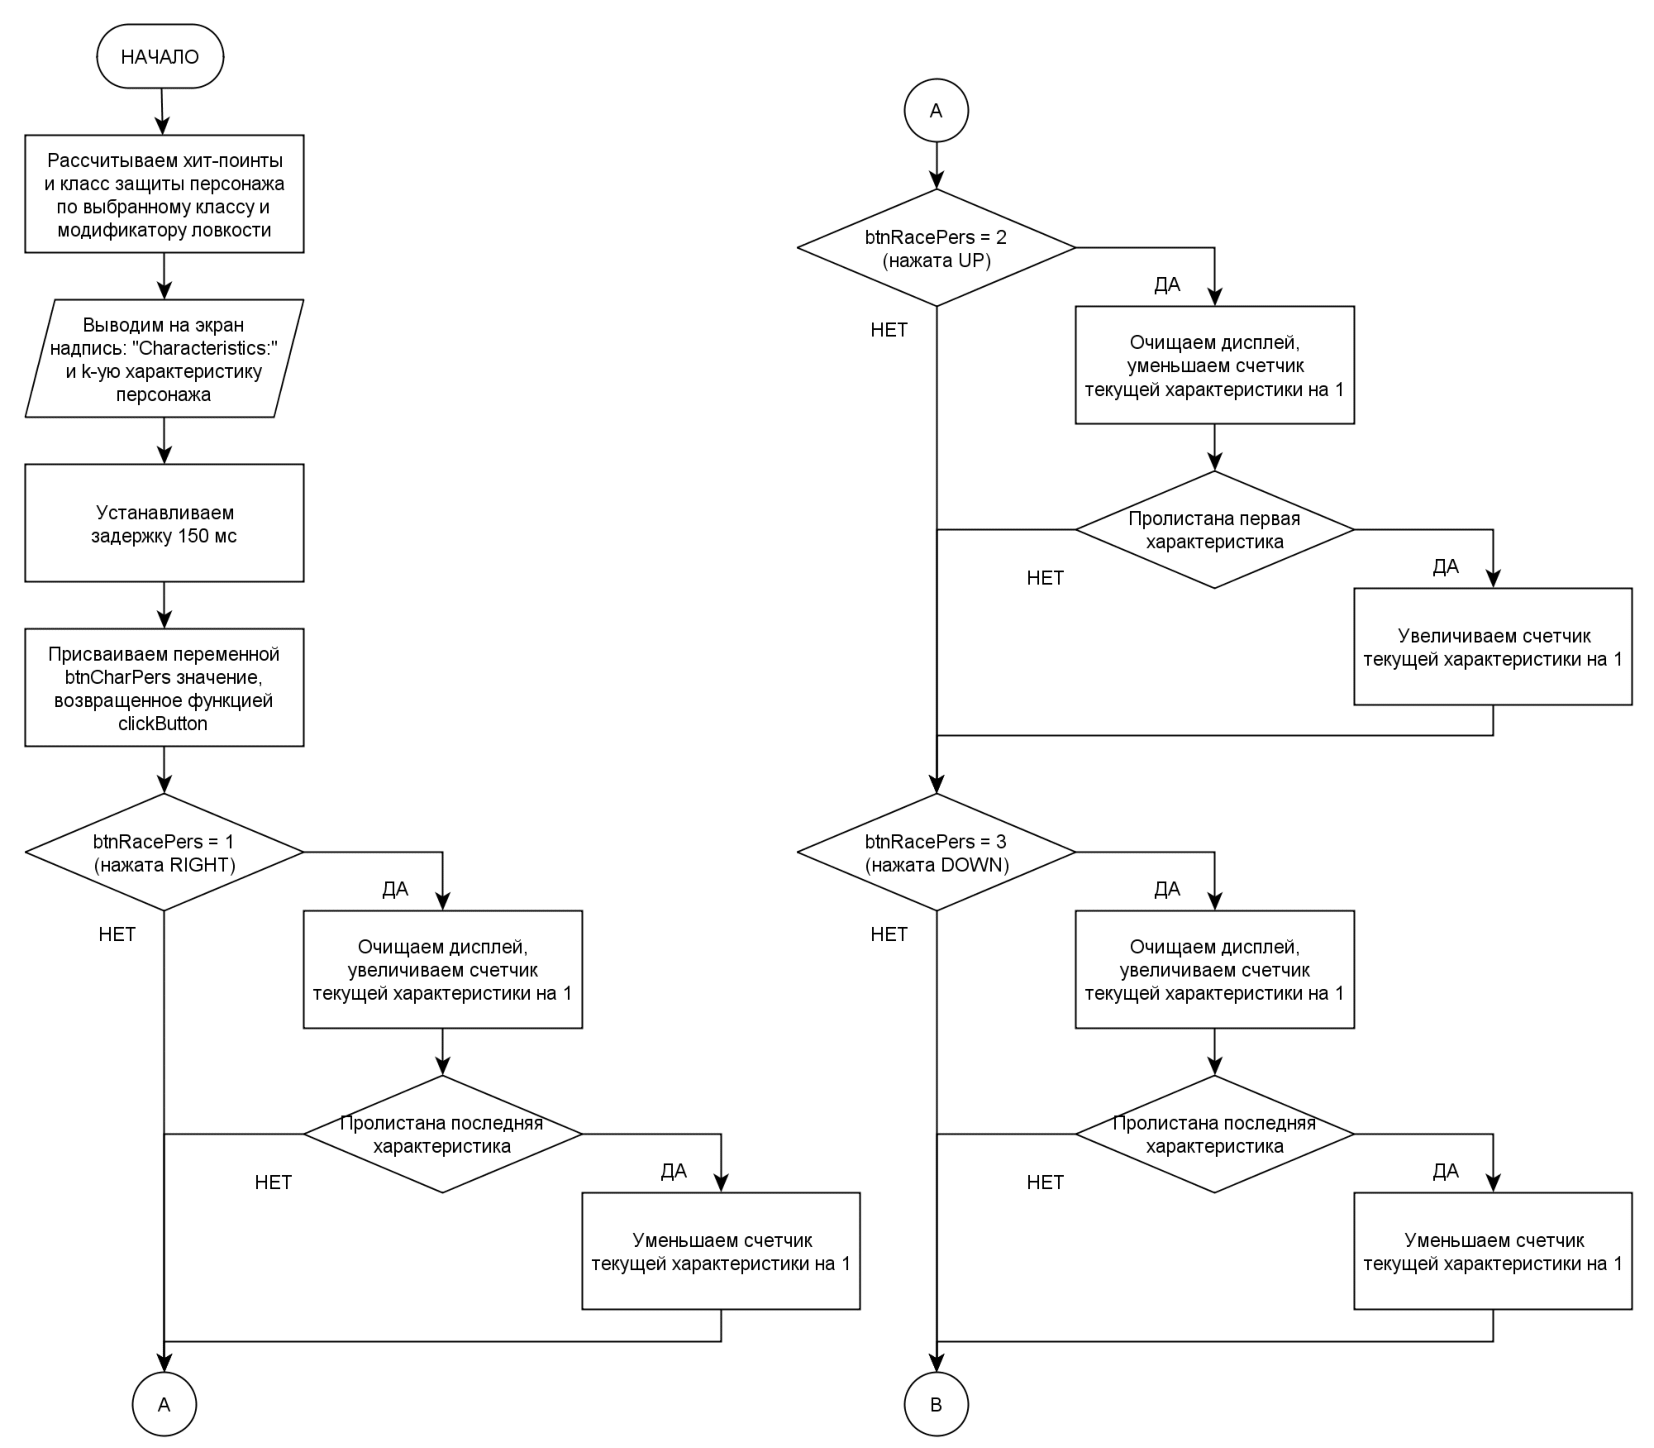
\includegraphics[scale=0.75]{charactPers1.png}
    \caption{Блок-схема функции charactPers.}
    \label{fig:char1}
\end{figure}

\begin{figure}[H]
    \centering
    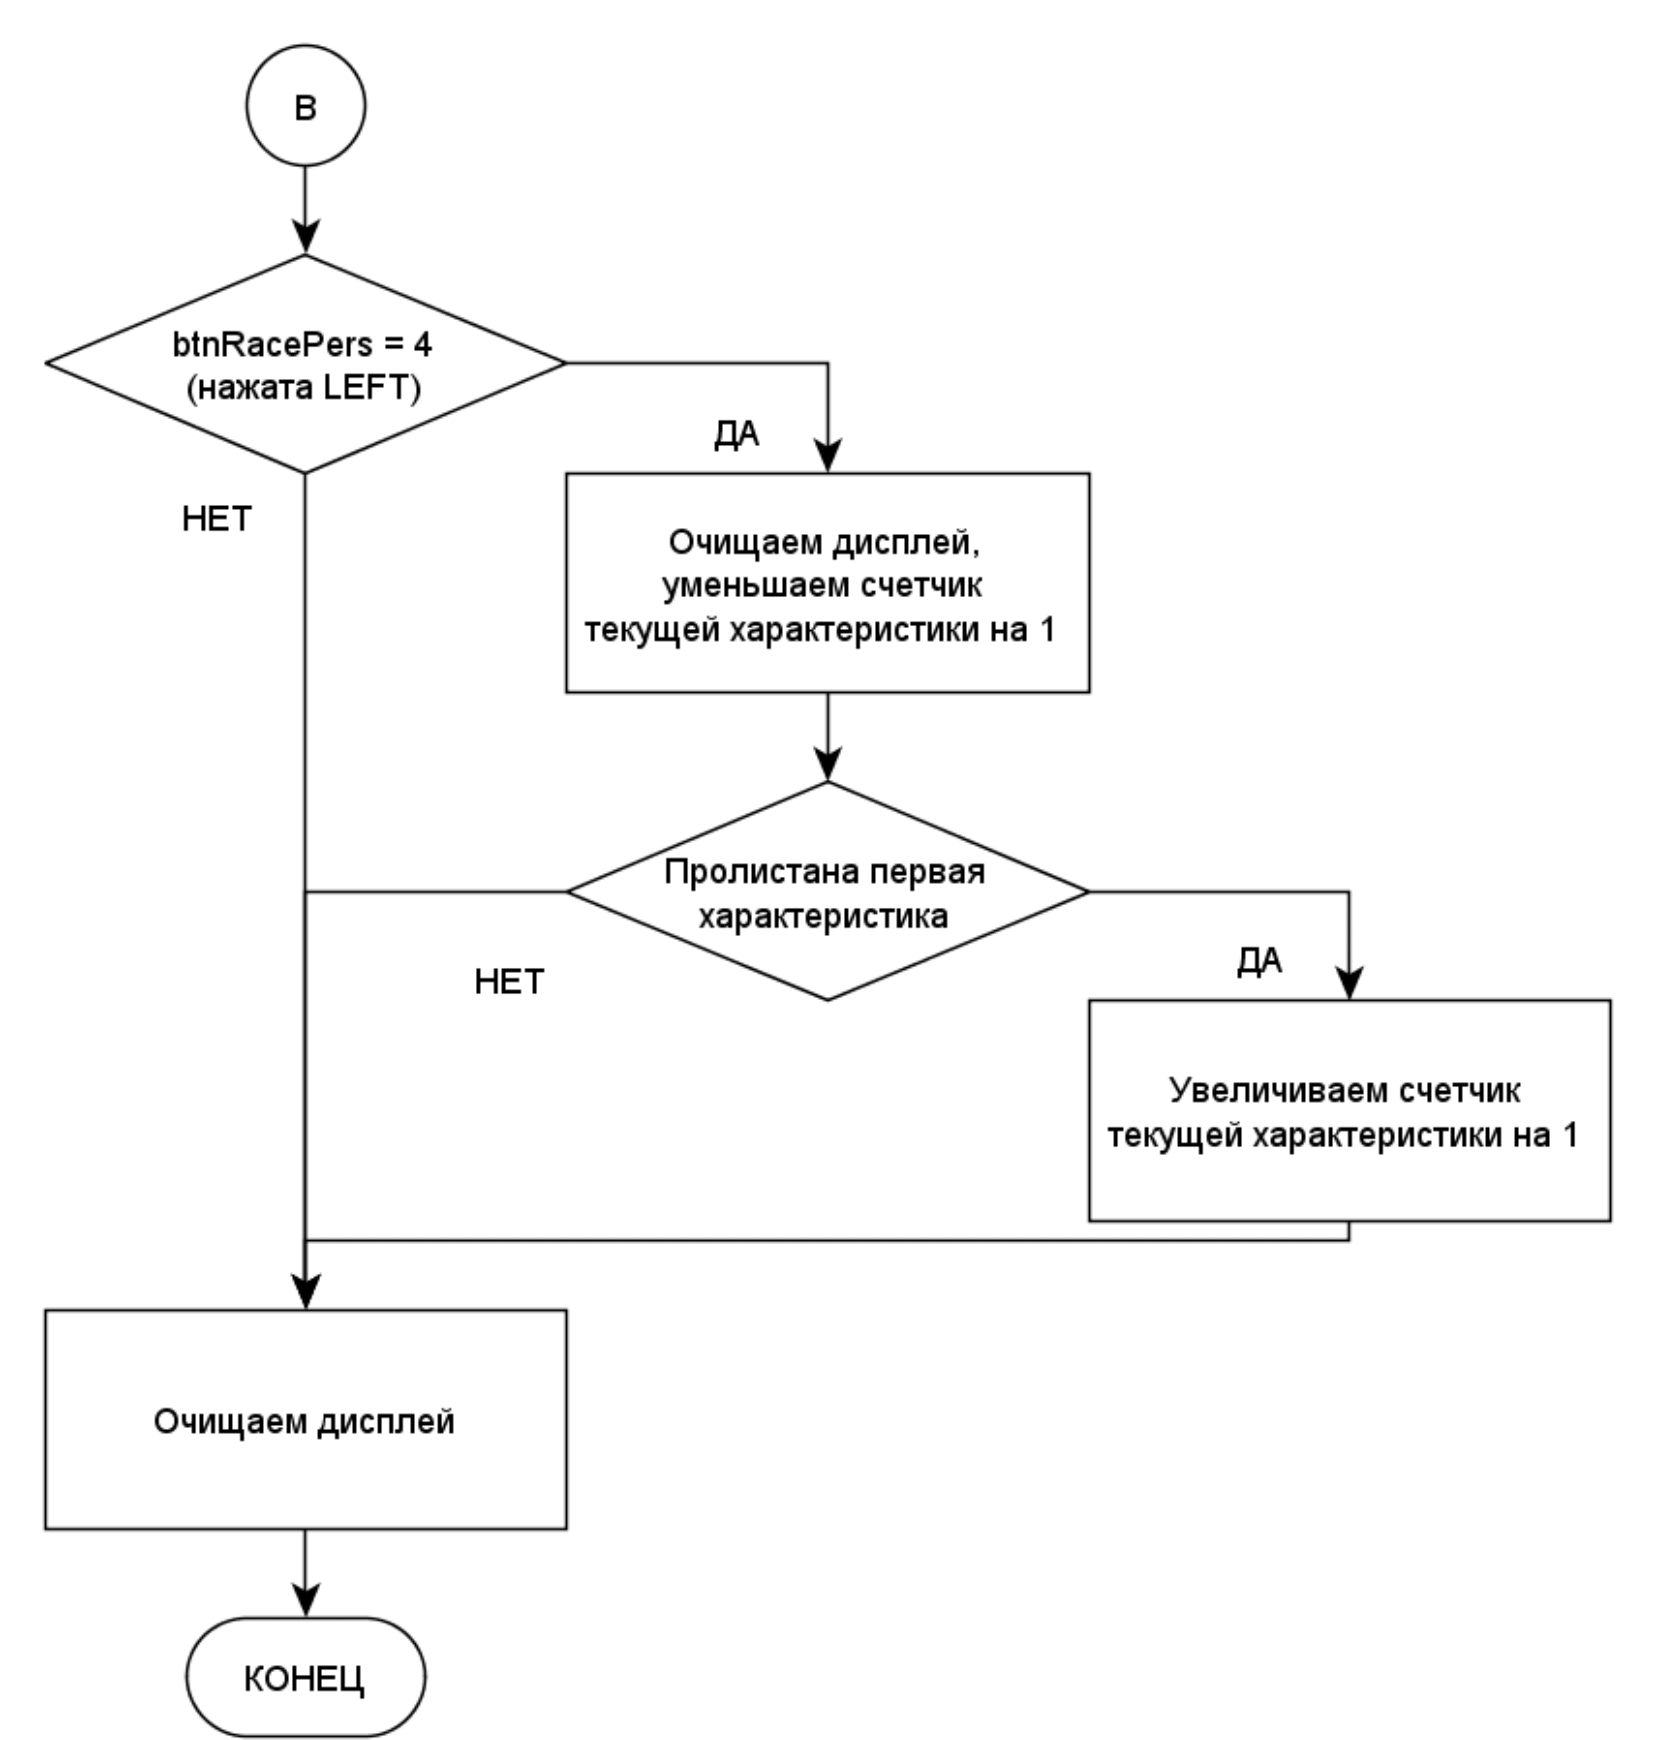
\includegraphics[scale=0.6]{charactPers2.png}
    \caption{Блок-схема функции charactPers.}
    \label{fig:char2}
\end{figure}

\subsection*{Функция clickButton}

Эта функция необходима для того, чтобы обрабатывать нажатия кнопок, она возвращает целое число, которое будет указывать на то, нажата ли кнопка и, если нажата, то какая. Блок-схема подпрограммы clickButton изображена на рис.~\ref{fig:click}.

\begin{figure}[H]
    \centering
    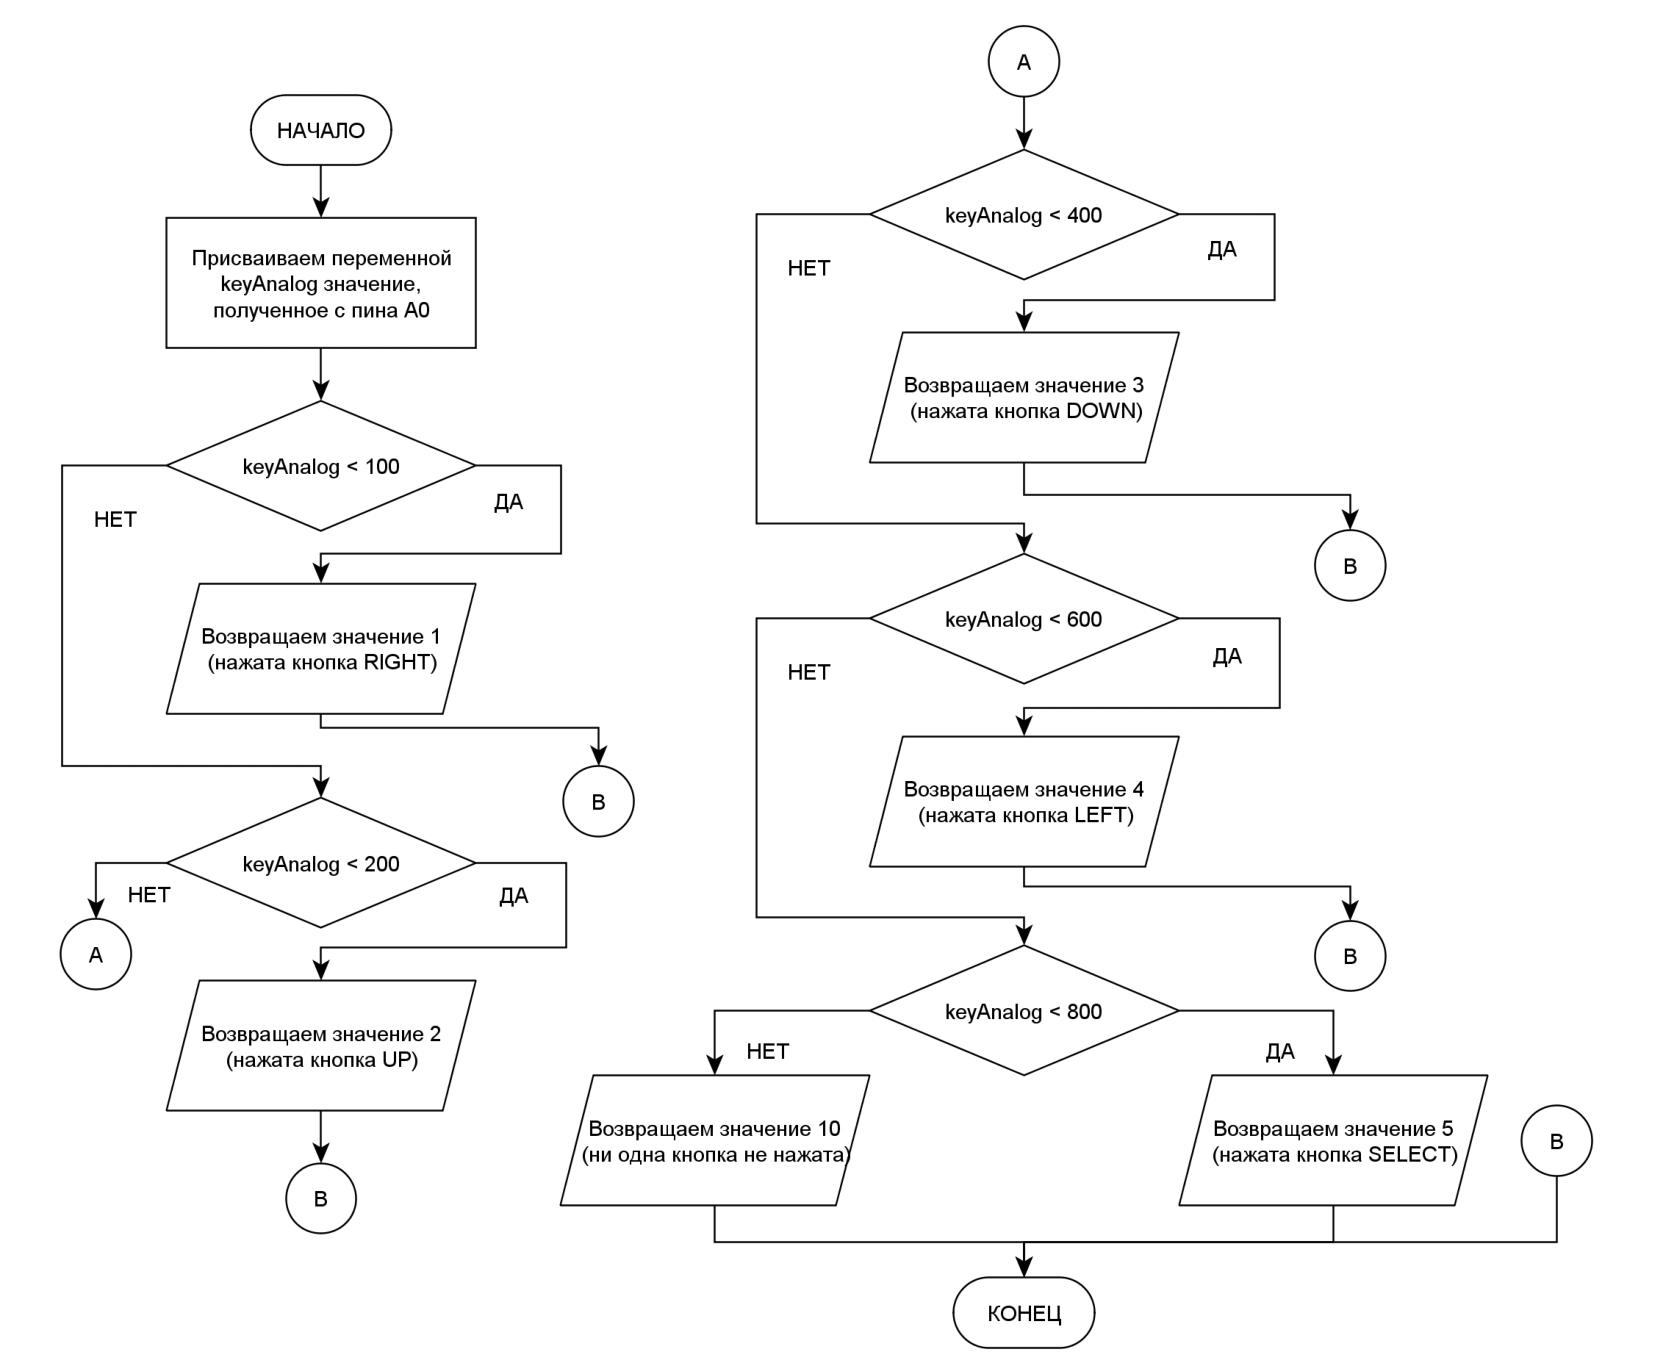
\includegraphics[scale=0.75]{clickButton.png}
    \caption{Блок-схема функции clickButton.}
    \label{fig:click}
\end{figure}

Помимо этих функций в проектах, написанных в Arduino IDE есть еще две стандартных функции. В функции setup задается скорость передачи данных для последовательного порта и инициализируется lcd-дисплей. В функции loop вызывается функция mainText для того, чтобы генератор персонажа работал вплоть до отключения его от питания. Блок-схемы алгоритмов подпрограмм loop и setup изображены на рис.~\ref{fig:setup},~\ref{fig:loop}.

\begin{figure}[H]
    \centering
    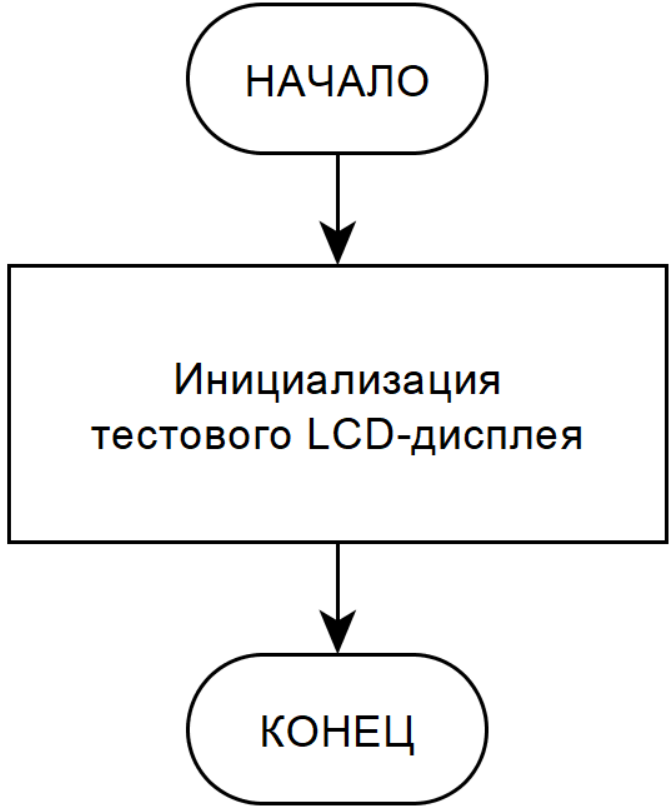
\includegraphics[scale=0.3]{setup.png}
    \caption{Блок-схема функции setup.}
    \label{fig:setup}
\end{figure}

\begin{figure}[H]
    \centering
    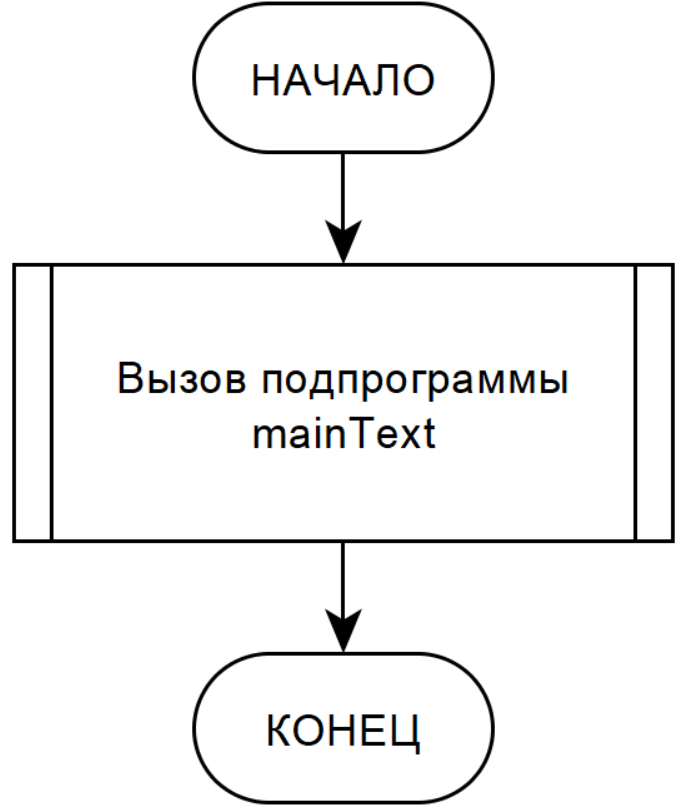
\includegraphics[scale=0.3]{loop.png}
    \caption{Блок-схема функции loop.}
    \label{fig:loop}
\end{figure}

\section{Разработка аппаратной части прототипа генератора персонажа D\&D}

Генератор персонажа реализован на отладочной плате Arduino Uno, в основе которой лежит микроконтроллер ATmega328. Для отображения меню генерации персонажа и навигации по нему используется плата расширения LCD Keypad Shield (Arduino-совместимая), на которой располагается LCD-дисплей 16x2, а также набор кнопок, которые могут быть использованы, непосредственно, для навигации. Разработка генератора персонажа велась с использованием интегрированной среды разработки Arduino IDE.

Для разработки прототипа устройства ключевым параметром является простота в исполнении, поэтому модульный способ конструирования с использованием отладочной платы и платы расширения к ней является предпочтительным, за счет своей простоты и удобства в сборке. Крепление платы расширения с дисплеем и кнопками осуществляется с помощью штыревых разъемов.

Для питания прототипа устройства используется внешний аккумулятор, для обеспечения относительной портативности.

\section{Отладка и тестирование работоспособности готового устройства для генерации персонажей D\&D}

Отладка программной части устройства проводилась в Arduino IDE. Основными аспектами отладки, помимо исправления синтаксических ошибок, являлись подстройка частоты обновления содержимого LCD-дисплея, а также борьба с дребезгом кнопок и случайными нажатиями, прощелкиваниями меню и других проблем, которые возникали с обработкой нажатий.

Ниже представлен скриншот успешной компиляции программы, после отладки.

\begin{figure}[H]
    \centering
    
\includegraphics[scale=0.5]{compile.png}
    \caption{Компиляция скетча.}
    \label{fig:compile}
\end{figure}

После того, как было получено сообщение об успешной компиляции прошивка была загружена в микроконтроллер.

Работоспособность устройства включала в себя проверку работы LCD-дисплея, кнопок и правильность реагирования на их нажатие.

Ниже будут представлены несколько фотографий, которые демонстрируют работу устройства.

Ниже главное окно генератора~\ref{fig:main_window}. Приветственный экран. Здесь контроллер ожидает, когда пользователь нажмет кнопку SELECT для начала генерации, на другие кнопки реакции не последует (исключение --- нажатие кнопки RESET).

\begin{figure}[H]
    \centering
    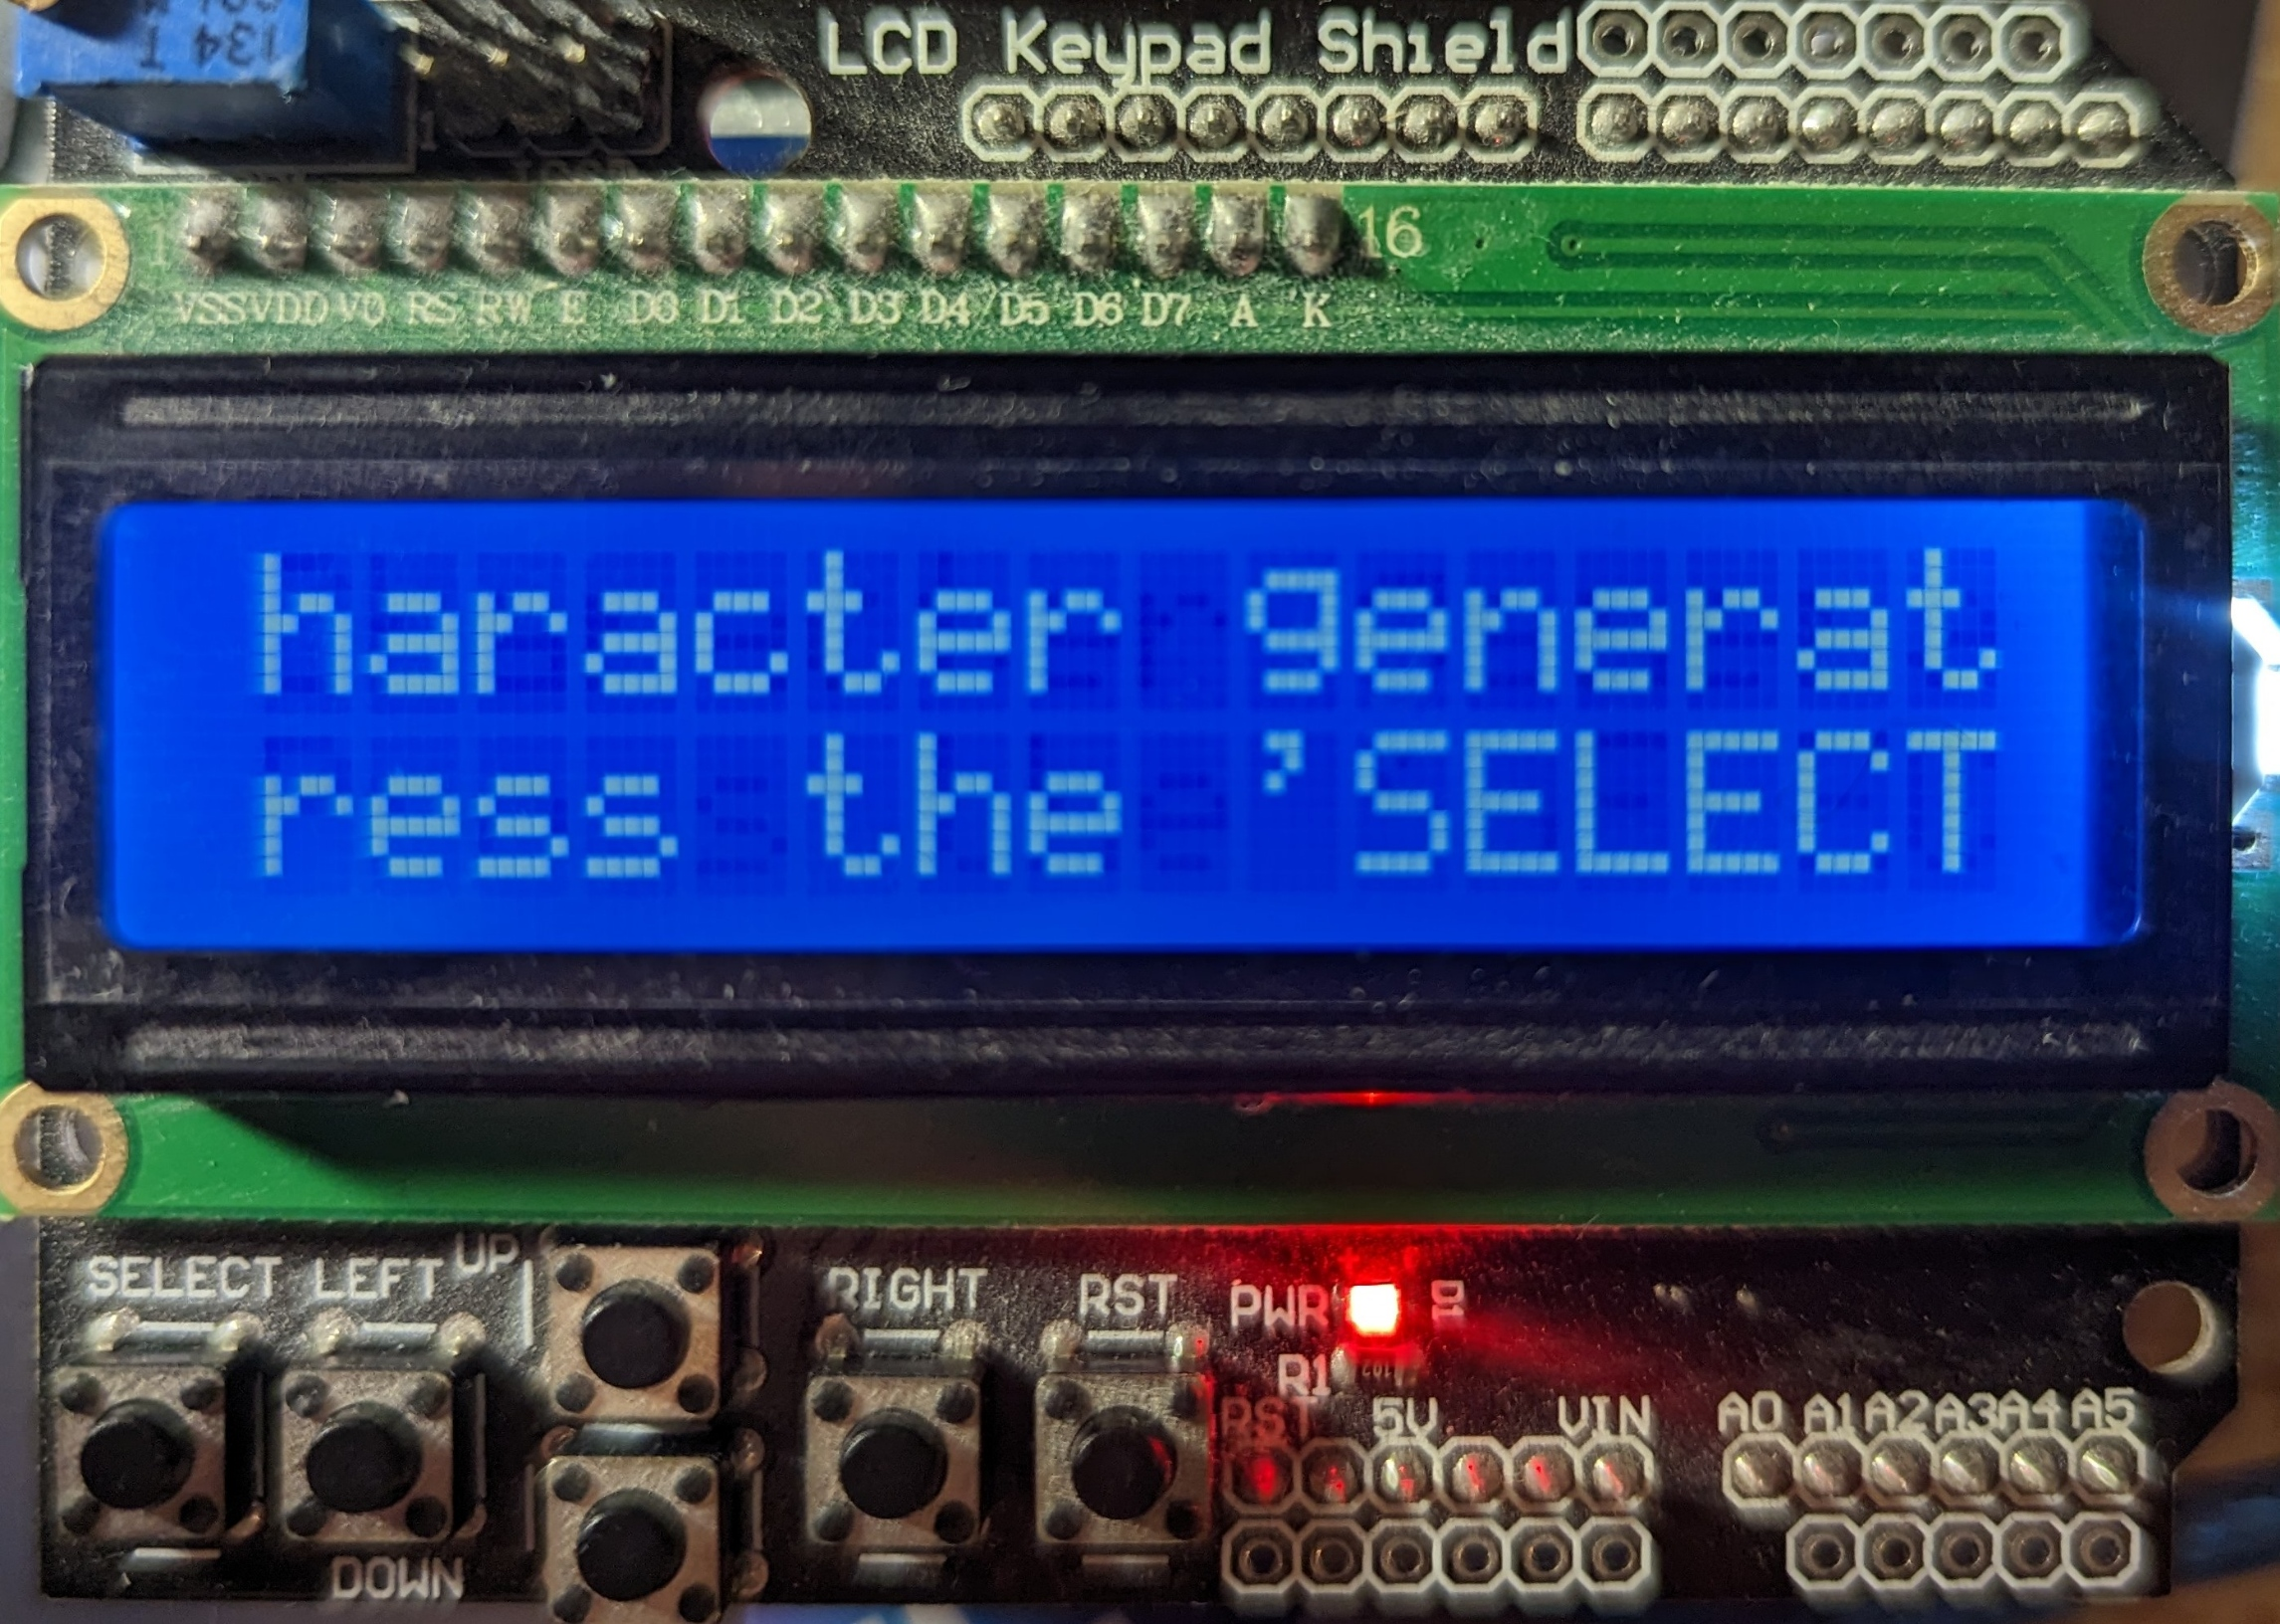
\includegraphics[scale=0.15]{mainWindow.jpg}
    \caption{Главный экран с бегущей строкой.}
    \label{fig:main_window}
\end{figure}

Эта часть меню представляет собой меню с примерами рас, которые доступны пользователю для выбора, для прокрутки по списку могут быть использованы четыре кнопки (LEFT и UP обеспечивают прокрутку вверх списка, RIGHT и DOWN --- вниз списка, соответственно)~\ref{fig:race}.

\begin{figure}[H]
    \centering
    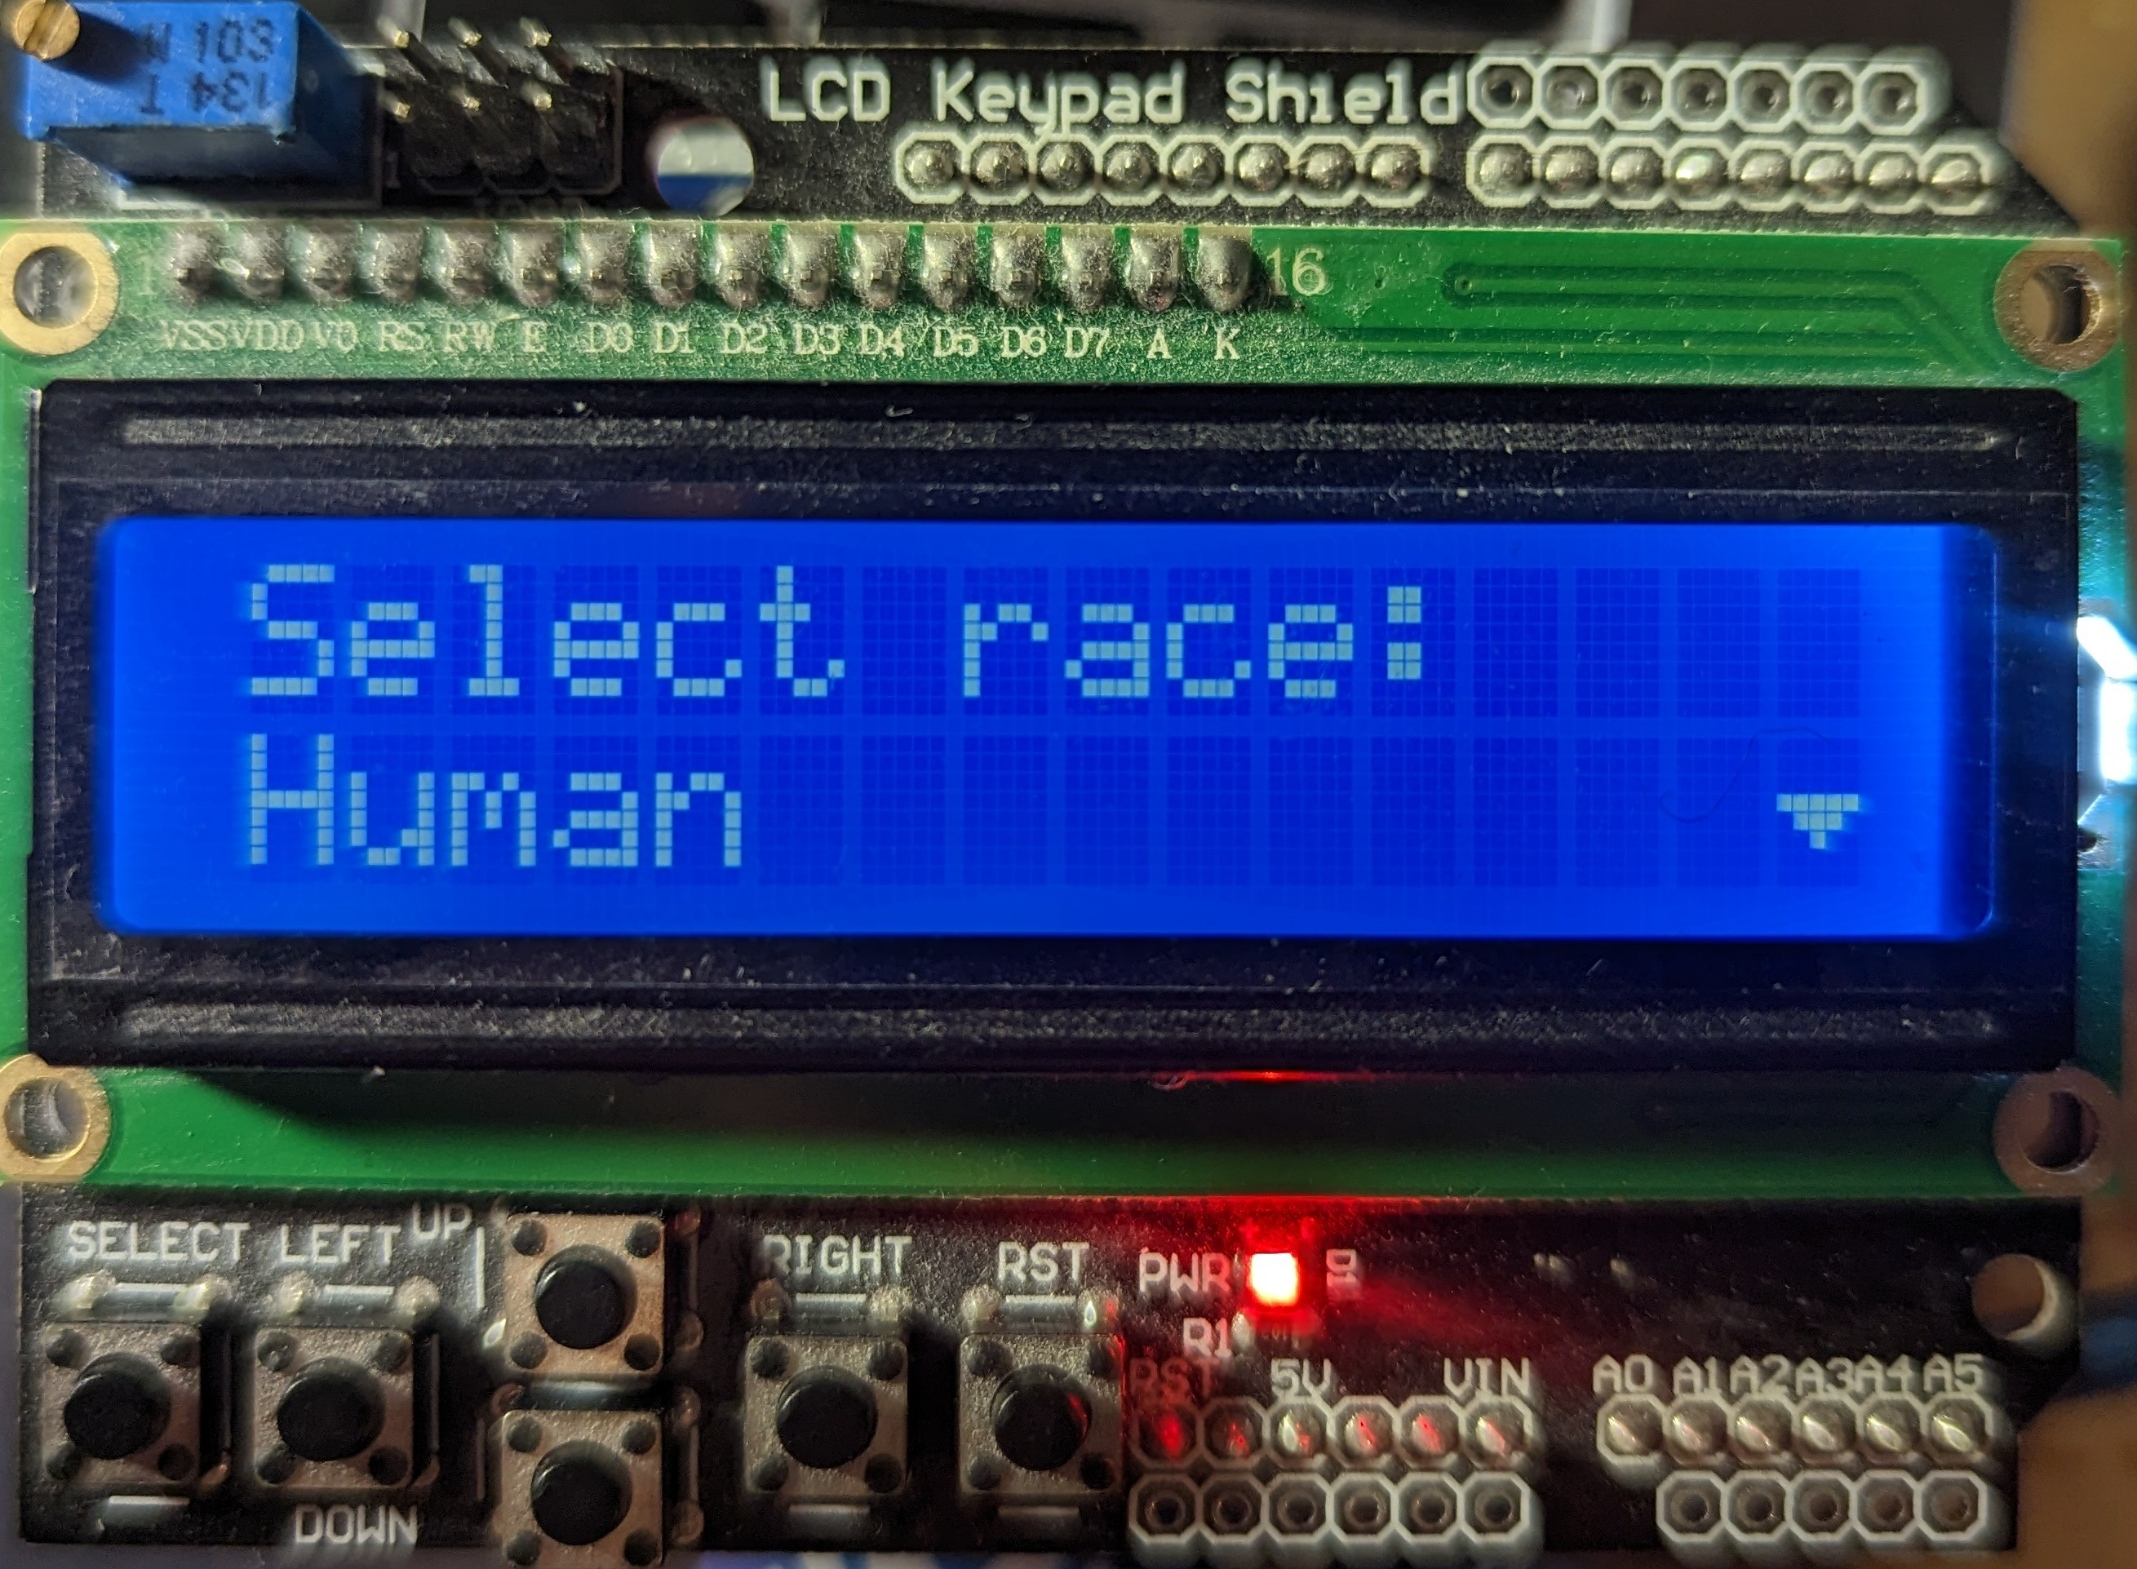
\includegraphics[scale=0.15]{selectRace.jpg}
    \caption{Выбор расы персонажа.}
    \label{fig:race}
\end{figure}

Данное меню для выбора класса персонажа идентично по принципу работы меню, которое используется для выбора класса~\ref{fig:class}. 

\begin{figure}[H]
    \centering
    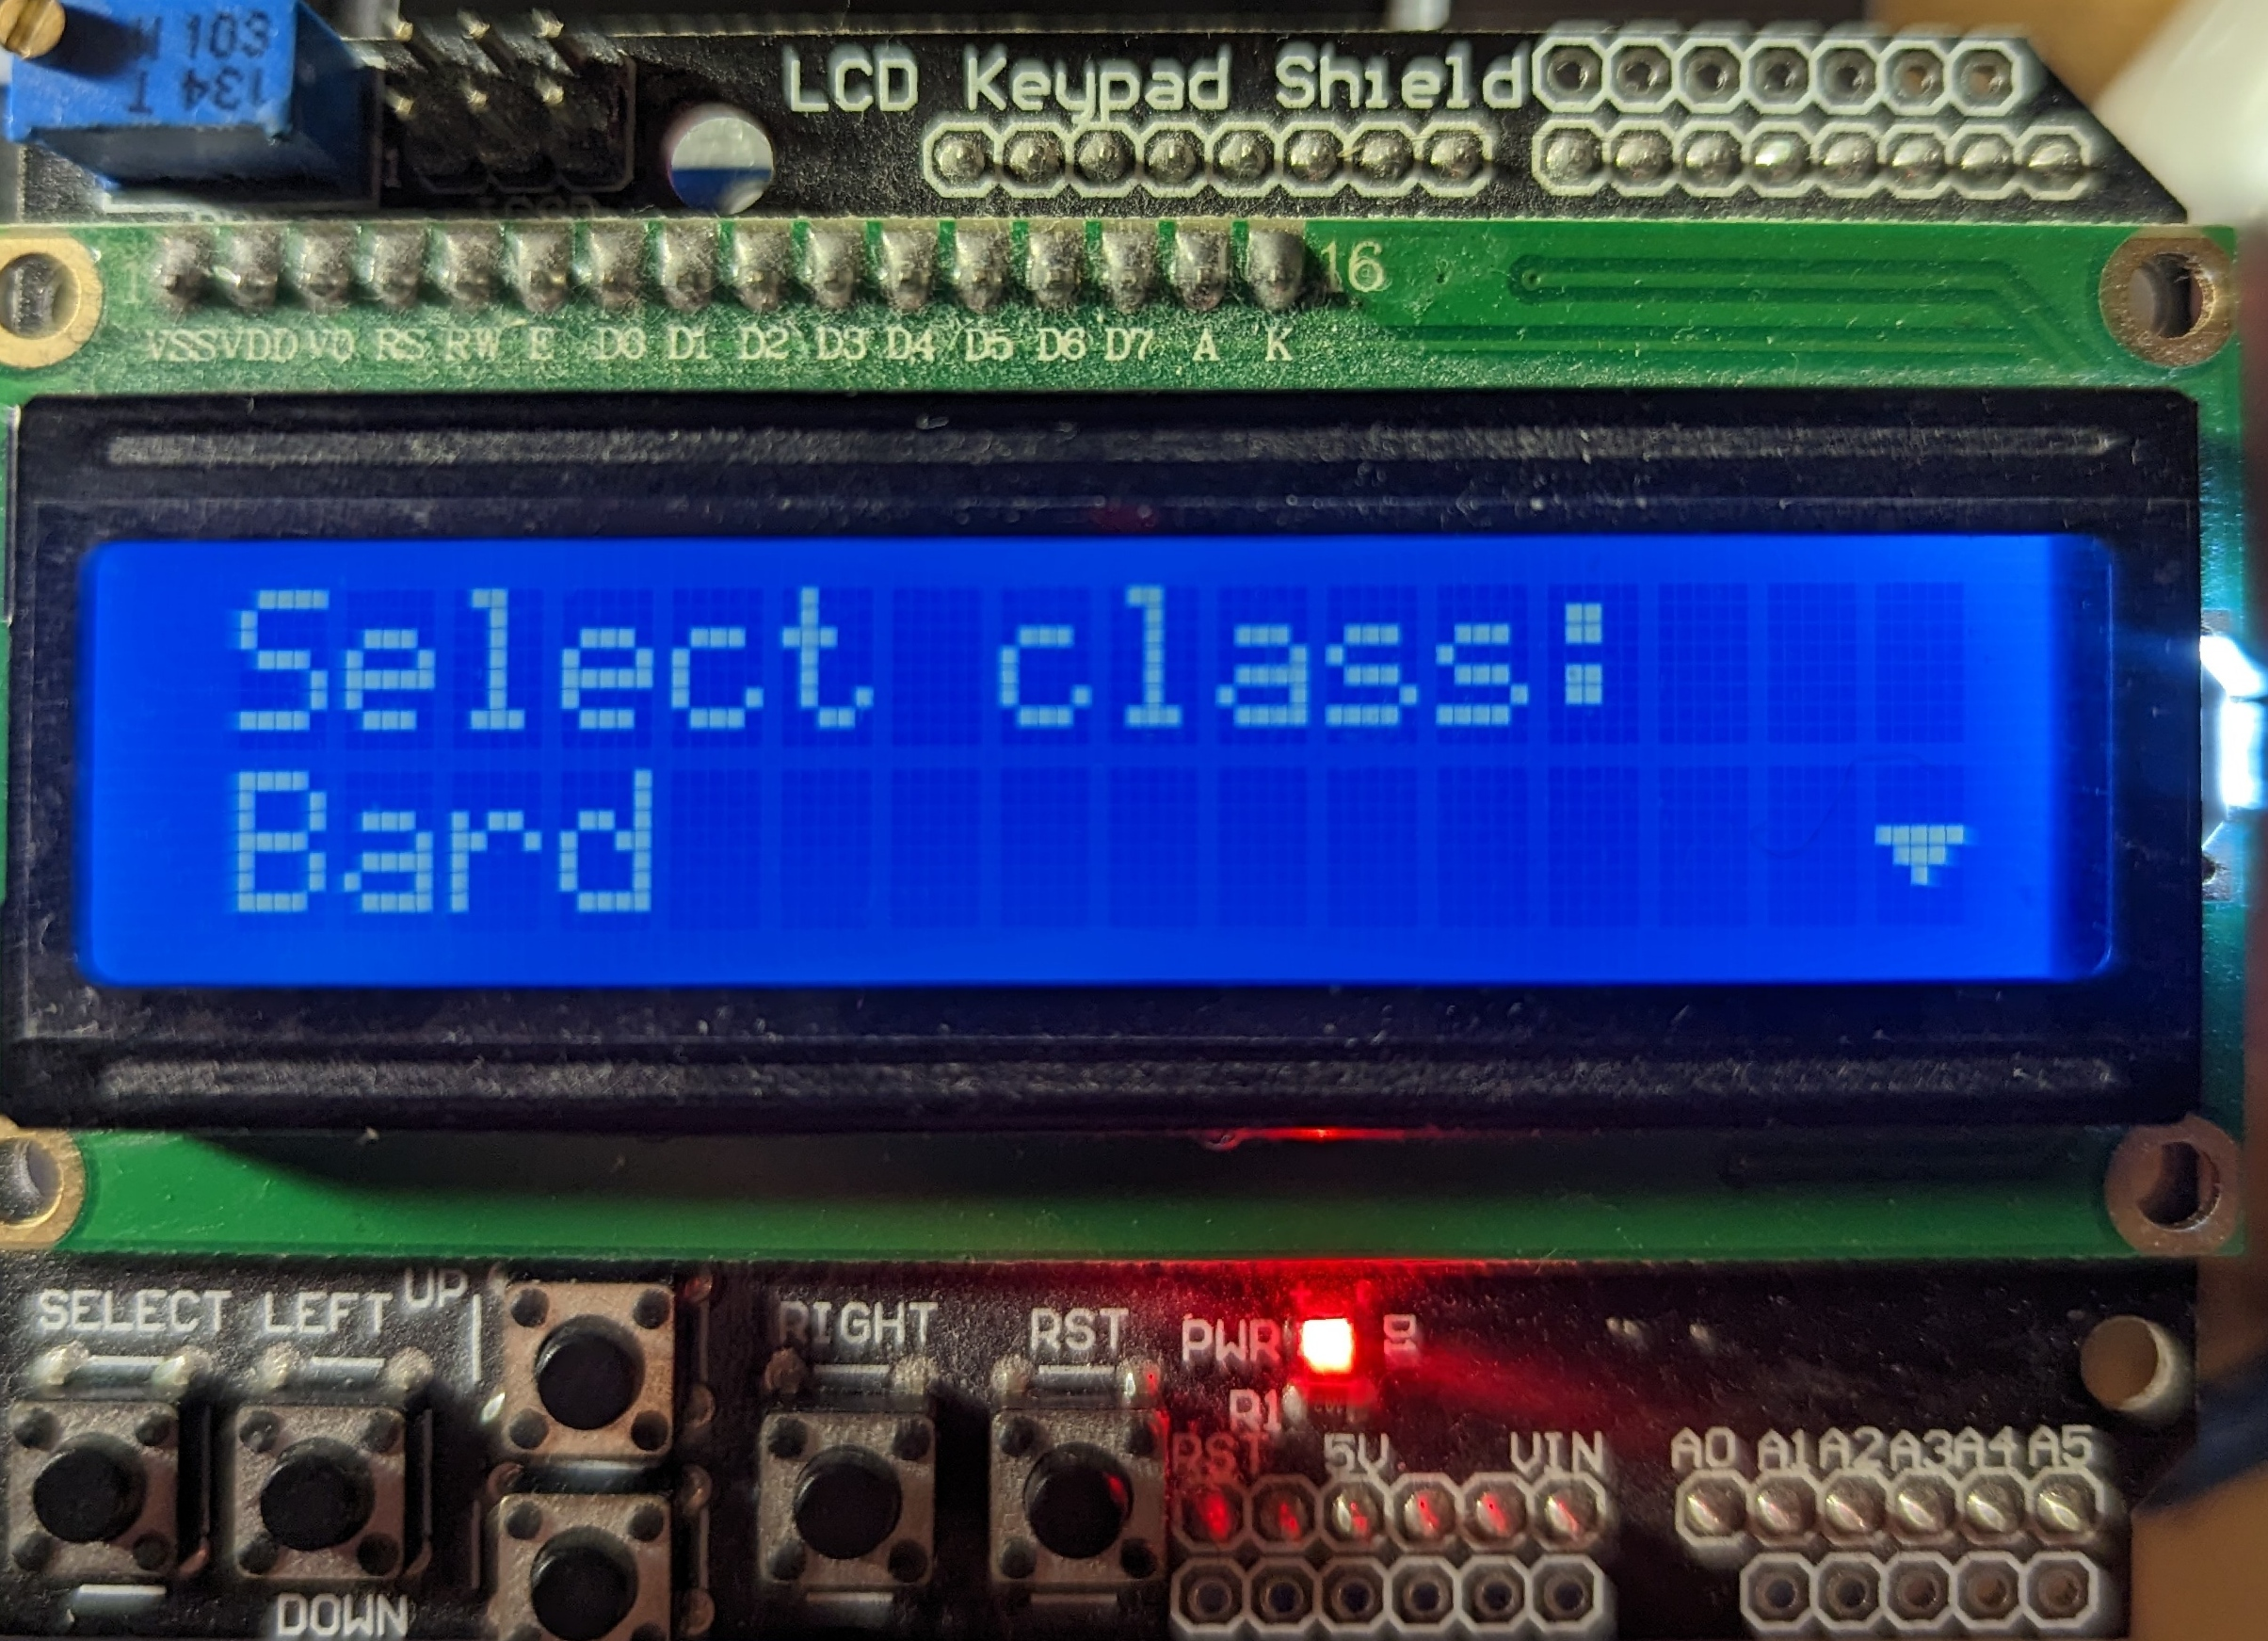
\includegraphics[scale=0.15]{selectClass.jpg}
    \caption{Выбор класса персонажа.}
    \label{fig:class}
\end{figure}

Данная область меню выводит пользователю данные о персонаже~\ref{fig:output}. Здесь пользователь может увидеть расу и класс, которые он выбрал на предыдущих шагах, а также сгенерированные базовые характеристики и некоторые дополнительные характеристики персонажа, такие как класс защиты и количество хит-поинтов персонажа.

\begin{figure}[H]
    \centering
    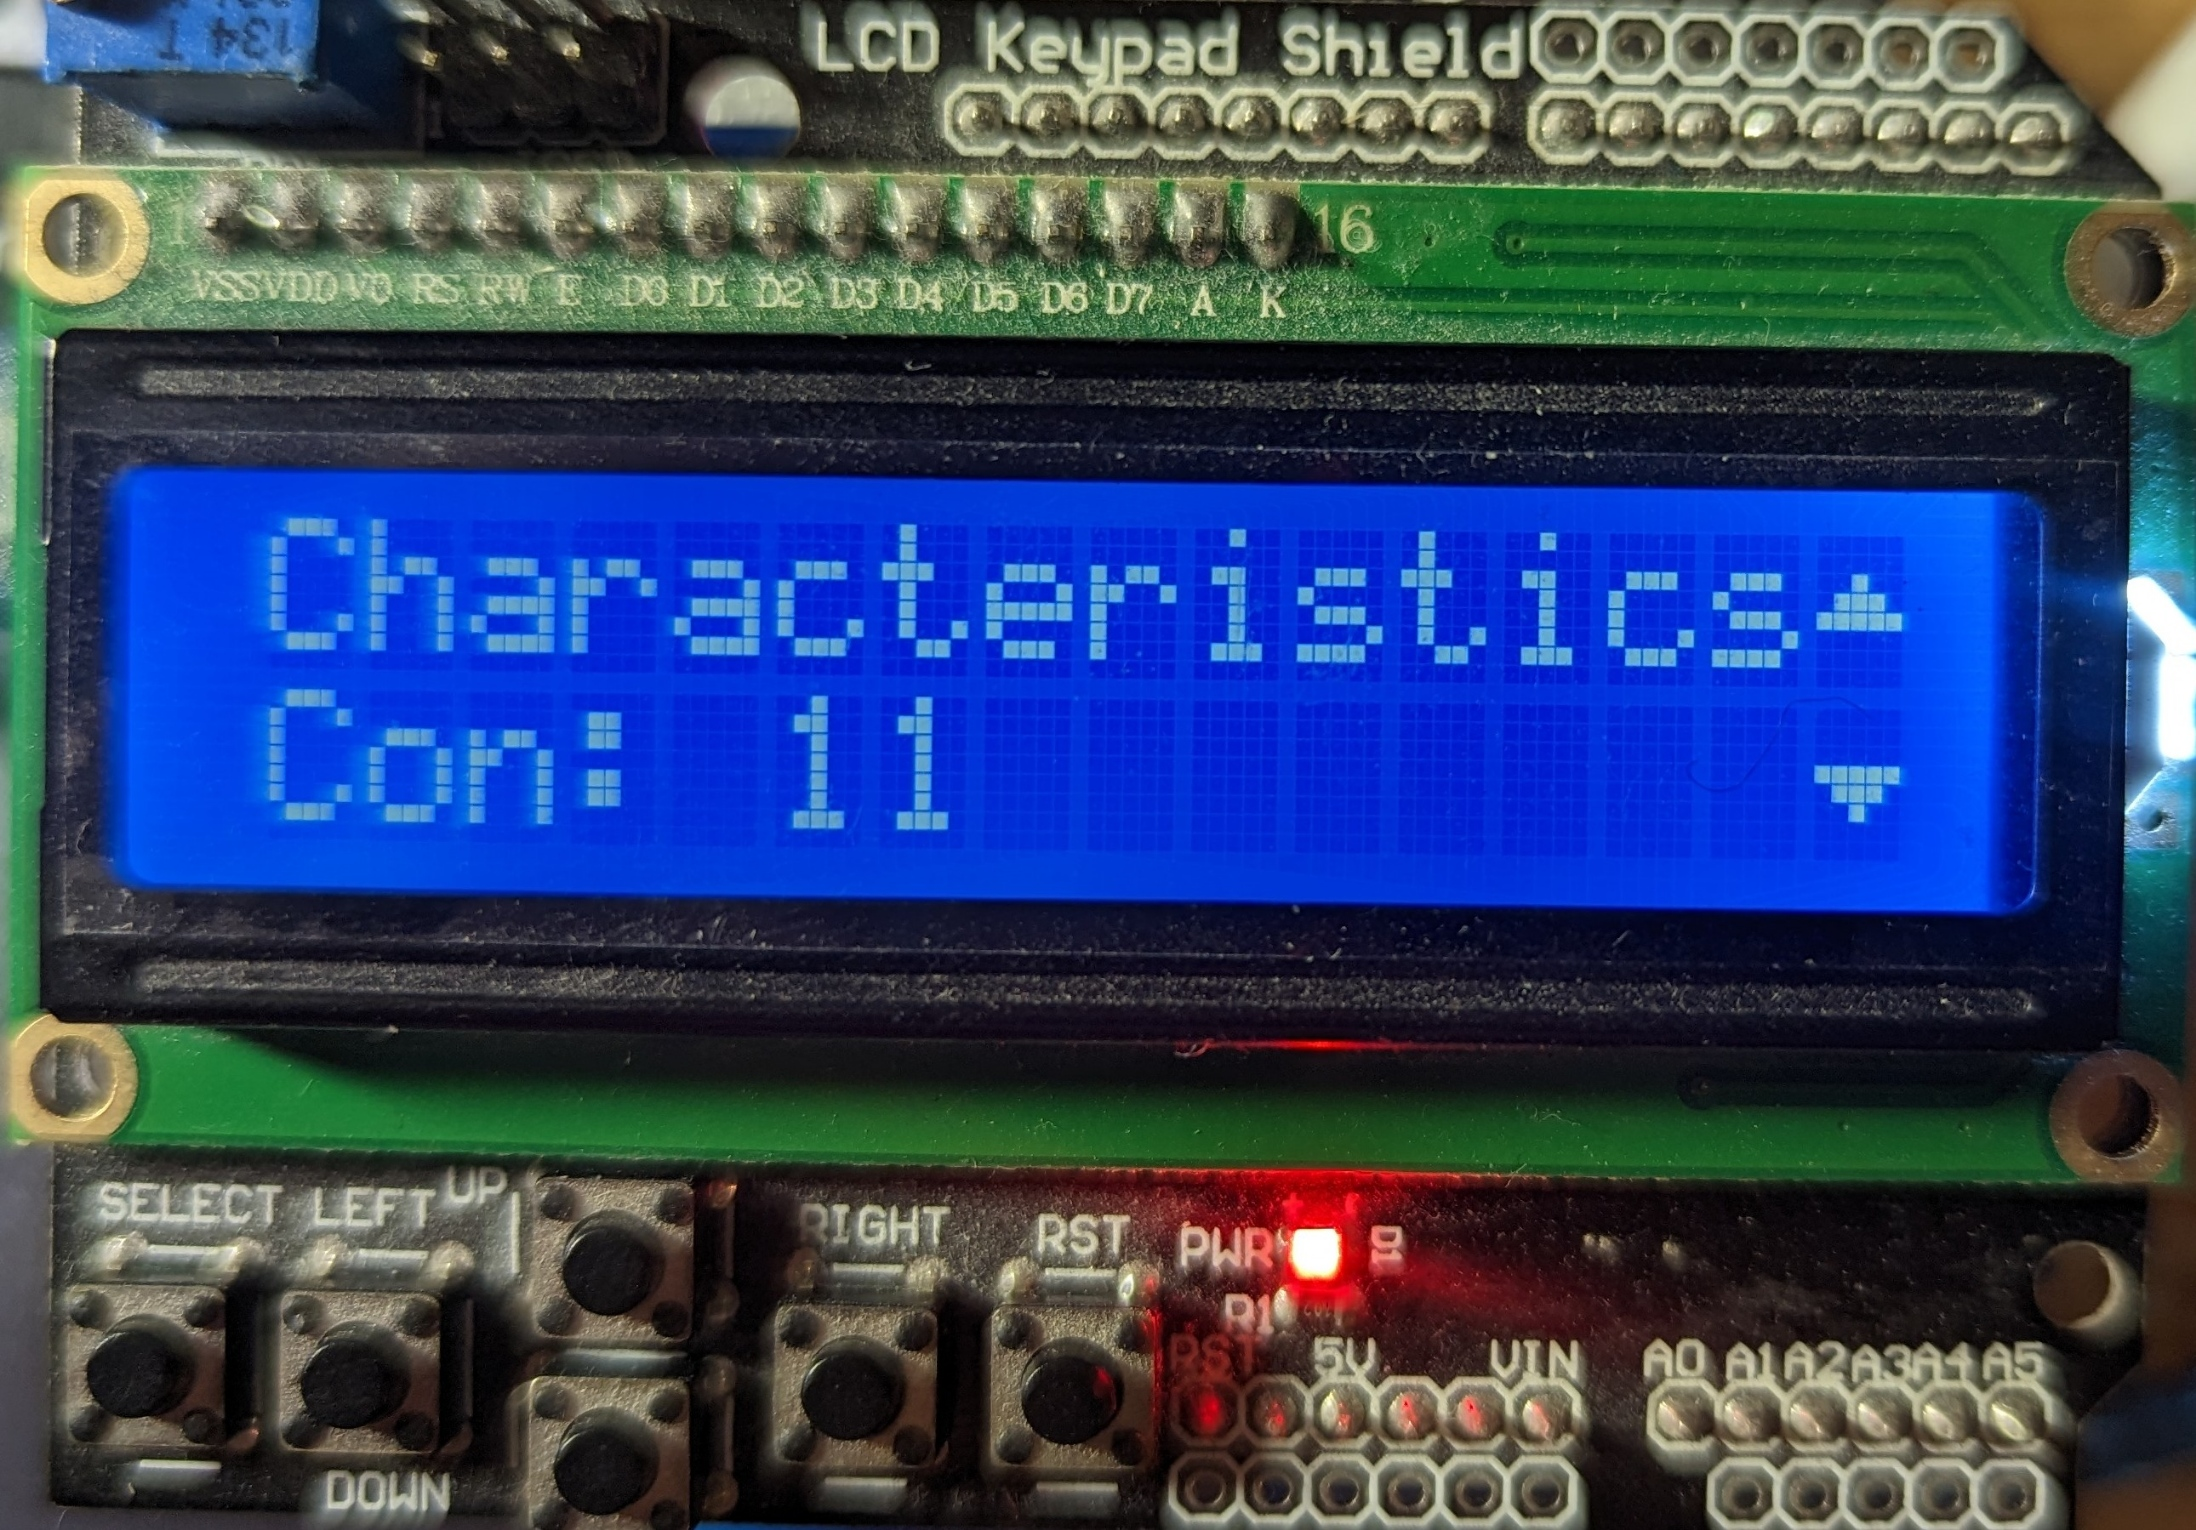
\includegraphics[scale=0.15]{output.jpg}
    \caption{Вывод итоговых характеристик.}
    \label{fig:output}
\end{figure}